\documentclass[xga]{xdvislides}
\usepackage[landscape]{geometry}
\usepackage{array}
\usepackage{graphics}
\usepackage{graphicx}
\usepackage{colordvi}
\usepackage{tabularx}
\usepackage{multirow}
\usepackage{fancyvrb}

\fvset{fontfamily=courier,commandchars=\\\{\}}

\newcommand{\smallish}{\fontsize{16}{16}\selectfont}

\begin{document}
\setfontphv

%%% Headers and footers
\lhead{\slidetitle}				% default:\lhead{\slidetitle}
\chead{CS615 - Aspects of System Administration}% default:\chead{\relax}
\rhead{Slide \thepage}				% default:\rhead{\sectiontitle}
\lfoot{\Gray{Review}}% default:\lfoot{\slideauthor}
\cfoot{\relax}					% default:\cfoot{\relax}
\rfoot{\Gray{\today}}

\vspace*{\fill}
\begin{center}
	\Hugesize
		CS615 - Aspects of System Administration\\ [1em]
		The Whole Semester In One Class\\ [1em]
	\hspace*{5mm}\blueline\\ [1em]
	\Normalsize
		Department of Computer Science\\
		Stevens Institute of Technology\\
		Jan Schaumann\\
		\verb+jschauma@stevens.edu+ \\
		\verb+https://www.cs.stevens.edu/~jschauma/615A/+
\end{center}
\vspace*{\fill}
%\setcounter{page}{0}
%\clearpage

\subsection{Basic Disk Concepts: Storage Models}
Direct Attached Storage (DAS)
\vfill
\begin{center}
	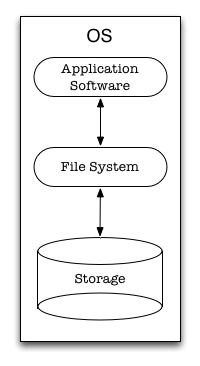
\includegraphics[scale=0.8]{pics/das.eps} \\
\end{center}
\verb+ssh lab 'df -hT /'+
\vfill

\subsection{Basic Disk Concepts: Storage Models}
Network Attached Storage (NAS)
\vfill
\begin{center}
	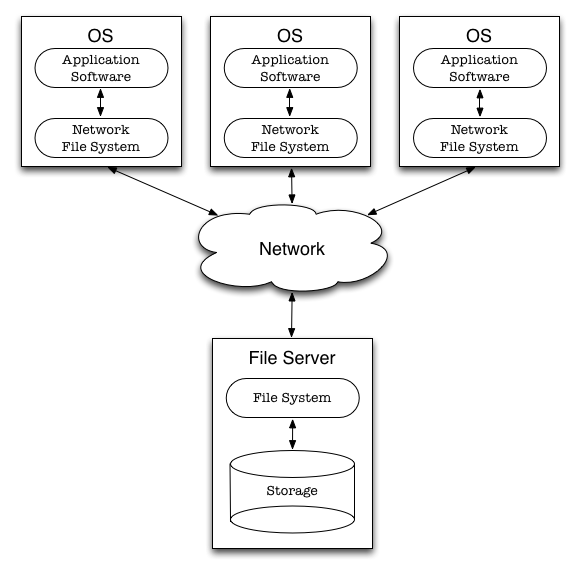
\includegraphics[scale=0.5]{pics/nas.eps} \\
\end{center}
\verb+ssh lab 'df -hT /home/$(whoami)'+
\vfill

\subsection{Basic Disk Concepts: Storage Models}
Storage Area Networks (SAN)
\vfill
\begin{center}
	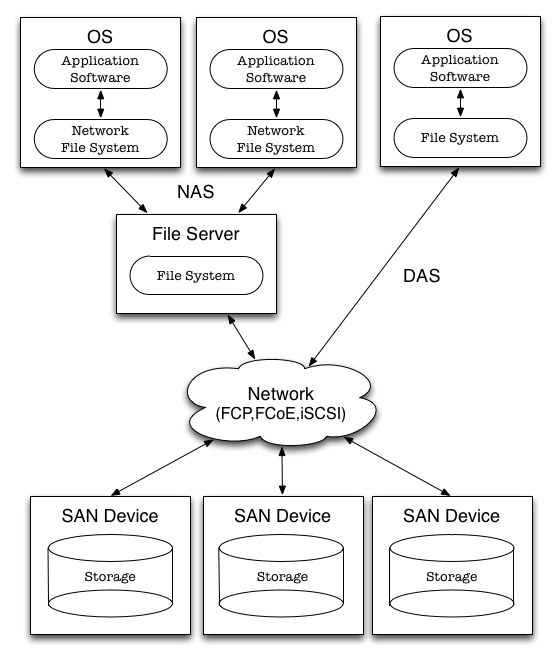
\includegraphics[scale=0.5]{pics/san-nas-das.eps} \\
\end{center}
\vfill

\subsection{Basic Disk Concepts: Storage Models}
Cloud Storage (Examples: EBS, S3)
\vfill
\begin{center}
	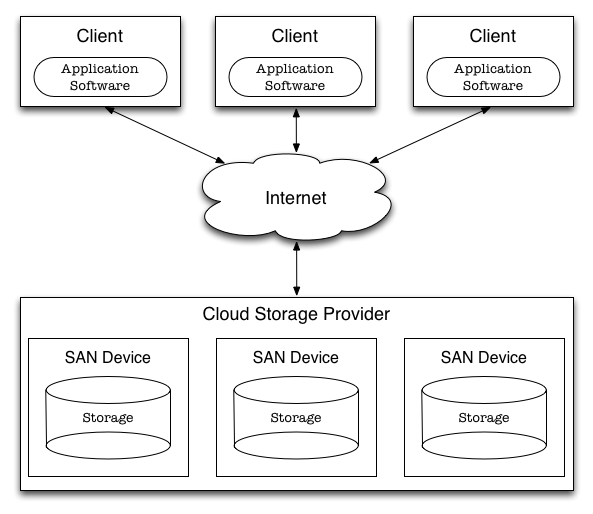
\includegraphics[scale=0.6]{pics/cloud-storage.eps} \\
\end{center}
\vfill

\subsection{Basic Disk Concepts: Disk Devices}
\vfill
	\begin{center}
		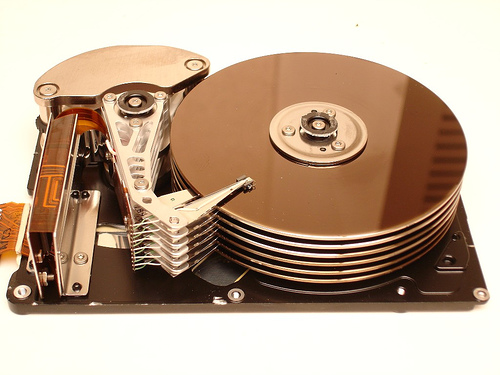
\includegraphics[scale=0.9]{pics/6platter.eps} \\
	\end{center}
\vfill

\subsection{Basic Disk Concepts: Physical Disk Structure}
\vfill
	\begin{center}
		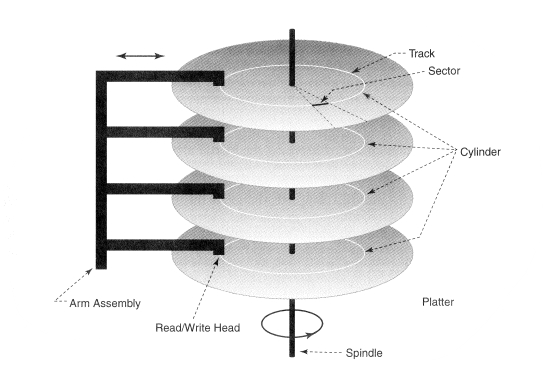
\includegraphics[scale=1.2]{pics/cylinders.eps} \\
	\end{center}
\vfill

\subsection{Basic Disk Concepts: Partitions}
NetBSD example (from {\tt disklabel(8)})

\begin{tabular}{ l l c }
Partition 'a': & / & \\
Partition 'b': & swap & \\
Partition 'e': & /home & \\
\end{tabular}

\begin{verbatim}
#        size    offset   fstype [fsize bsize cpg/sgs]
a:  20972385        63   4.2BSD   4096 32768  1180  # (Cyl.      0*- 20805)
b:   1048320  20972448     swap                     # (Cyl.  20806 - 21845)
c:  78140097        63   unused      0     0        # (Cyl.      0*- 77519)
d:  78140160         0   unused      0     0        # (Cyl.      0 - 77519)
e:  56119392  22020768   4.2BSD   4096 32768 58528  # (Cyl.  21846 - 77519)
\end{verbatim}

\subsection{Basic Filesystem Concepts: The UNIX Filesystem}
\vspace*{\fill}
\begin{center}
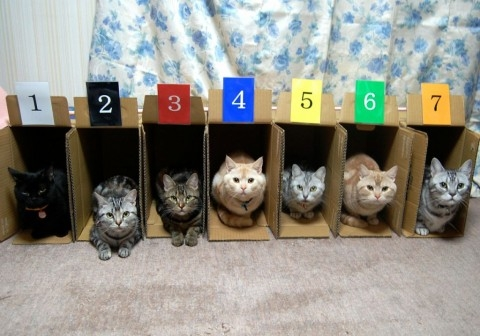
\includegraphics[scale=1.0]{pics/numbered-cats.eps} \\
\end{center}
\vspace*{\fill}

\subsection{Basic Filesystem Concepts: The UNIX Filesystem}
The filesystem is responsible for storing the data on the disk.
So to read/write data, it needs to know in which physical blocks the actual
data is located; ie how to map files to the disk blocks.
\\

Components of the Berkeley Fast Filesystem:
\\

\newcolumntype{S}{>{\centering\arraybackslash} m{.4\linewidth} }
\begin{tabular}{ p{10cm} S }
\begin{itemize}
	\item set of {\em inode} storage cells
	\item set of scattered ``superblocks''
	\item map of disk blocks
	\item block usage summary
	\item set of data blocks
\end{itemize}
& \multirow{2}{*}{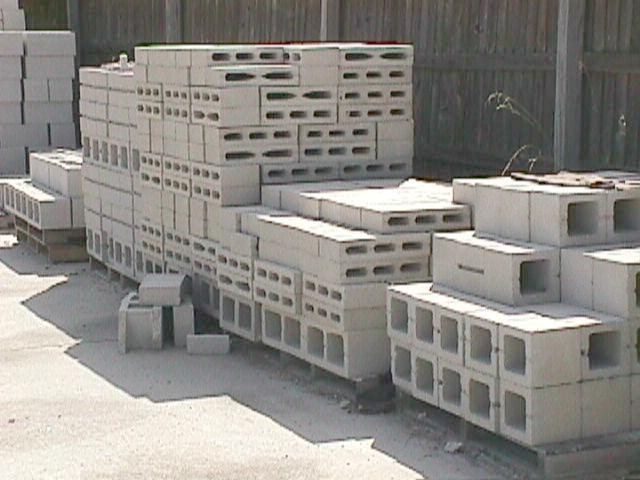
\includegraphics[scale=0.3]{pics/block.eps}} \\
\end{tabular}

\subsection{Basic Filesystem Concepts: The UNIX Filesystem}
\begin{center}
	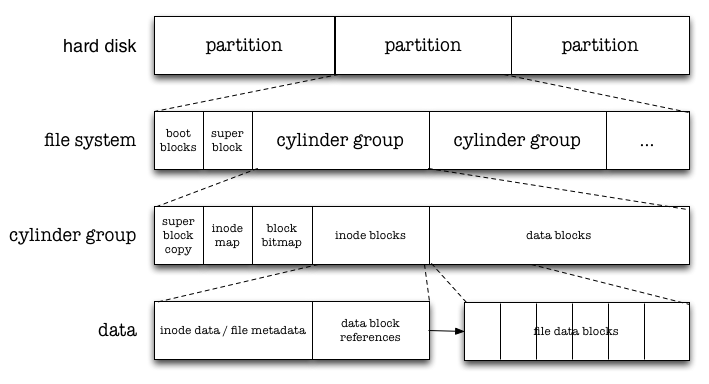
\includegraphics[scale=0.8]{pics/ufs-details.eps} \\
\end{center}
\vspace*{\fill}

\subsection{Basic Filesystem Concepts: The UNIX Filesystem}
Information stored in an {\em inode}:
\begin{itemize}
	\item user owner and group owner ID's
	\item file type
	\item access mode (permissions)
	\item file access and modification time
	\item file status modification time
	\item number of links to the file
	\item size of the file
	\item disk device containing this file
\end{itemize}

\begin{verbatim}
$ stat /etc/passwd
\end{verbatim}

\newpage
\vspace*{\fill}
\begin{center}
    \Hugesize
        Lecture 03 \\ [1em]
    \hspace*{5mm}
    \blueline\\
    \hspace*{5mm}\\
	Software Installation Concepts
\end{center}
\vspace*{\fill}

\subsection{Down the stack we go}
Consider a website on an AWS EC2 instance...
\\

...it might:

\begin{itemize}
	\item require a web server
	\item require PHP, Perl, Ruby, Javascript, ...
	\item which uses generic library functions
	\item which make various system calls
	\item which the kernel handles for the OS
	\item which is running in a virtual machine
	\item which is running on top of a hypervisor
	\item which uses firmware to manage various components
	\item which is running on some hardware
\end{itemize}

\subsection{...and back up again}
Bringin up this web service might include...
\\

\begin{itemize}
	\item power on hardware
	\item POST and other firmware initialization
	\item first stage boot loader
	\item second stage boot loader
	\item hypervisor kernel dom0 starts
	\item domU is started
	\item guest OS kernel starts
	\item kernel initializes (virtual) hardware
	\item {\tt init(8)} (or similar) starts
	\item system processes / daemons start
	\item web server runs, binds network socket, serves content
\end{itemize}

\subsection{Types of Software}
\vfill
\begin{center}
	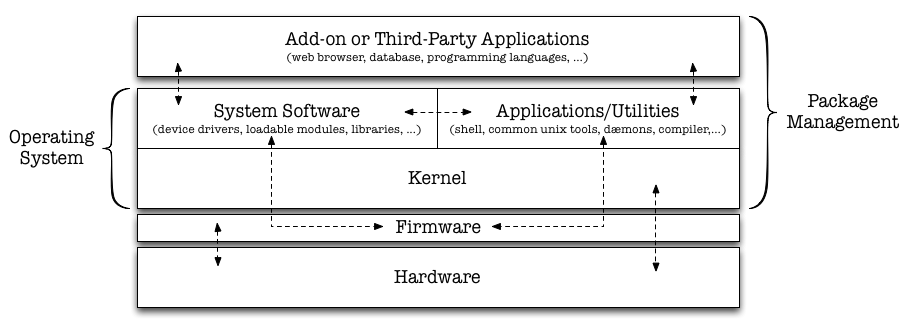
\includegraphics[scale=0.8]{pics/types-of-software.eps}
\end{center}
\vfill

\subsection{Base OS Installation}
General steps:
\begin{itemize}
	\item boot from boot media (CD, network, ...)
	\item identify root device
	\item optionally identify additional devices
	\item create partition table / disklabel
	\item create filesystem(s)
	\item install MBR, bootblocks etc.
	\item install / copy / extract OS
	\item optionally add application software
	\item perform basic system configuration
	\item reboot
\end{itemize}

\subsection{OS Installation}
\small
\begin{verbatim}
# fdisk -f -u 0 -s 169/63/4194241 /dev/rwd0d
# fdisk -f -c /usr/mdec/mbr /dev/rwd0d
# fdisk -f -a -0 /dev/rwd0d
# disklabel -e -I wd0
[...]
4 partitions:
#      size   offset fstype [fsize bsize cpg/sgs]
a:  4194241       63 4.2BSD    0     0      0 # (Cyl.      0*- 4161*)
c:  4194241       63 4.2BSD    0     0      0 # (Cyl.      0*- 4161*)
d:  4194304        0 unused    0     0      0 # (Cyl.      0 - 4161*)
# /sbin/newfs -O 2 /dev/rwd0a
/dev/rwd0a: 2048.0MB (4194240 sectors) block size 16384,
        fragment size 2048 using 12 cylinder groups of
        170.67MB, 10923 blks, 21504 inodes.
super-block backups (for fsck_ffs -b #) at:
32, 349568, 699104, 1048640, 1398176, 1747712, 2097248, 2446784,
....................................................................
# mount -o async /dev/wd0a /mnt
# for pkg in base comp etc games man misc modules text kern-GENERIC; do
tar zxpf /i386/binary/sets/${pkg}.tgz -C /mnt
done
# cp /mnt/usr/mdec/boot /mnt/boot
# /usr/sbin/installboot -v -o timeout=5 /dev/rwd0a \
        /mnt/usr/mdec/bootxx_ffsv2
File system:       /dev/rwd0a
Primary bootstrap: /usr/mdec/bootxx_ffsv2
Boot options:      timeout 5, flags 0, speed 9600, ioaddr 0, console pc
# cd /mnt/dev && ./MAKEDEV all
# shutdown -r now
\end{verbatim}
\Normalsize

\subsection{System Software vs. Third Party Software}
Consider:
\begin{itemize}
	\item OS upgrades vs. software upgrades
	\item location of configuration files
	\item duplicates or conflicting versions in the base system vs. the
		add-ons
	\item startup scripts, d{\ae}mons
	\item location of third party software
	\item dependencies
	\item installation by hand and/or installation using a package manager
	\item proprietary third party software
\end{itemize}

\newpage
\vspace*{\fill}
\begin{center}
    \Hugesize
        Lecture 04 \\ [1em]
    \hspace*{5mm}
    \blueline\\
    \hspace*{5mm}\\
	Multiuser Fundamentals
\end{center}
\vspace*{\fill}

\subsection{Implications of a Multi-User System}
\begin{itemize}
	\item users may want to keep files private
	\item users may want to share files
	\item users may (try to gain) access to files they shouldn't have access to
	\item users may (want to) do things that affect other users
	\item different users may require different privileges
\end{itemize}

\subsection{Authentication}

\begin{itemize}
	\item proof of identity, not proof of {\em authorization}
	\item something you know, something you have, something you are
	\item multi-factor authentication combines these to help protect against different threats
	\item mutual authentication may be a requirement
\end{itemize}

\subsection{Authentication}
Common examples:
\begin{itemize}
	\item passwords, PINs
	\item ssh keys, PGP keys, X.509 certificates
	\item security tokens: OTPs in hardware or software, RFIDs
	\item physical biometrics: fingerprint, retina scan, facial recognition
	\item behavioral biometrics: speech pattern, gait, keystroke dynamics...
\end{itemize}
\vspace{.5in}

Mix and match the above to yield multi-factor
authentication:
\begin{itemize}
	\item password + PIN via e.g. SMS
	\item ssh key + TOTP from e.g. mobile device
	\item fingerprint + security token
	\item ...
\end{itemize}


\newpage
\vspace*{\fill}
\begin{center}
    \Hugesize
        Lecture 05 / Lecture 06 \\ [1em]
    \hspace*{5mm}
    \blueline\\
    \hspace*{5mm}\\
	Networking
\end{center}
\vspace*{\fill}

\subsection{Subnets}
\begin{verbatim}
$ ipcalc -n 155.246.89.100/16
Address:   155.246.89.100       10011011.11110110. 01011001.01100100
Netmask:   255.255.0.0 = 16     11111111.11111111. 00000000.00000000
Wildcard:  0.0.255.255          00000000.00000000. 11111111.11111111
=>
Network:   155.246.0.0/16       10011011.11110110. 00000000.00000000
HostMin:   155.246.0.1          10011011.11110110. 00000000.00000001
HostMax:   155.246.255.254      10011011.11110110. 11111111.11111110
Broadcast: 155.246.255.255      10011011.11110110. 11111111.11111111
Hosts/Net: 65534                 Class B
\end{verbatim}
\vspace{.5in}
Try also: \verb+sipcalc -a 155.246.89.100/16+

\subsection{IPv6 Subnets}
\begin{verbatim}
$ sipcalc 2001:470:30:84:e276:63ff:fe72:3900/64
-[ipv6 : 2001:470:30:84:e276:63ff:fe72:3900/64] - 0

[IPV6 INFO]
Expanded Address        - 2001:0470:0030:0084:e276:63ff:fe72:3900
Compressed address      - 2001:470:30:84:e276:63ff:fe72:3900
Subnet prefix (masked)  - 2001:470:30:84:0:0:0:0/64
Address ID (masked)     - 0:0:0:0:e276:63ff:fe72:3900/64
Prefix address          - ffff:ffff:ffff:ffff:0:0:0:0
Prefix length           - 64
Address type            - Aggregatable Global Unicast Addresses
Network range           - 2001:0470:0030:0084:0000:0000:0000:0000 -
                          2001:0470:0030:0084:ffff:ffff:ffff:ffff

\end{verbatim}

\subsection{Mommy, where do IP addresses come from?}
\vspace*{\fill}
\begin{center}
The Internet Assigned Numbers Authority (IANA) oversees global IP
address/AS number allocation, root zone management etc. \\
	\vspace{.5in}
	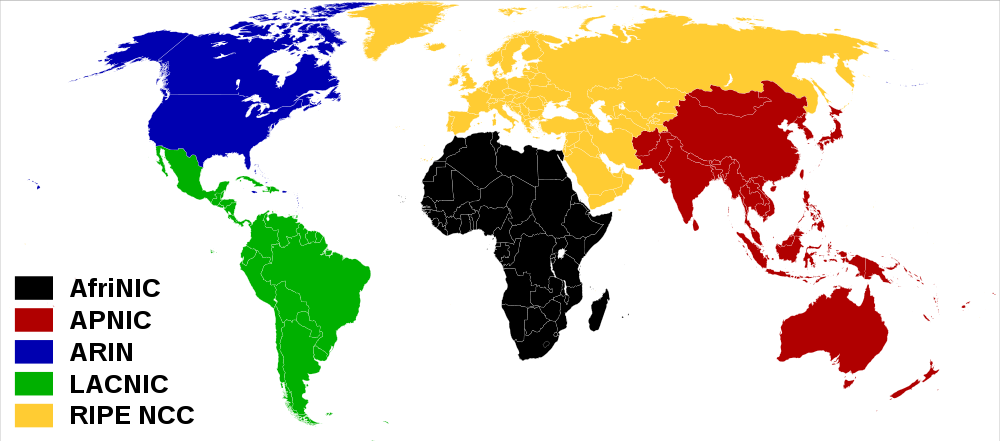
\includegraphics[scale=0.4]{pics/rirs.eps} \\
	\vspace{.5in}
	Regional Internet Registries (RIR) manage the allocation and
registration of Internet number resources within a region of the world.
\end{center}
\vspace*{\fill}

\subsection{WHOIS ASN?}
Autonomous System Numbers (ASNs) are assigned by IANA
to the RIRs, see e.g. {\tt
ftp://ftp.arin.net/pub/stats/arin/}
\\

You can query databases on the internet about e.g. IP
block or ASN information via the {\tt WHOIS} protocol:

\begin{verbatim}
$ whois 155.246.89.100 | more
NetRange:       155.246.0.0 - 155.246.255.255
CIDR:           155.246.0.0/16
NetName:        STEVENS
NetHandle:      NET-155-246-0-0-1
Parent:         NET155 (NET-155-0-0-0-0)
NetType:        Direct Assignment
Organization:   Stevens Institute of Technology (SIT)
RegDate:        1991-12-31
Updated:        2007-01-29
Ref:            https://whois.arin.net/rest/net/NET-155-246-0-0-1
\end{verbatim}

\subsection{WHOIS ASN?}
Carriers connect their Autonomous Systems at {\em
Internet Exchange Points} (IXPs) to route traffic
between the different networks.\\

This {\em peering} happens amongst carriers on a
tiered basis. \\

Examples:
\begin{verbatim}
https://peeringdb.com/net?asn=6939
https://peeringdb.com/net/27
https://peeringdb.com/net/433
https://peeringdb.com/net/457
\end{verbatim}

\subsection{Networking}
Stringing cables across the oceans' floors since 1866!
\vspace*{\fill}
\begin{center}
	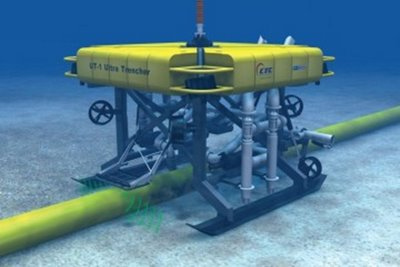
\includegraphics[scale=1.0]{pics/internet-undersea-cable.eps} \\
	\verb+http://www.submarinecablemap.com/+ \\
	\verb+http://is.gd/CjanOu+
\end{center}
\vspace*{\fill}

\subsection{Networking}
The internet is a physical place. \\
\begin{center}
\vspace*{\fill}
	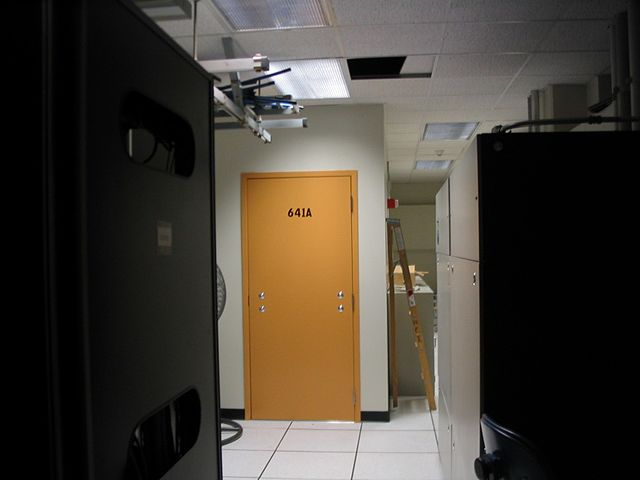
\includegraphics[scale=0.6]{pics/Room_641A.eps} \\
\vspace*{\fill}
{\tt https://en.wikipedia.org/wiki/Room\_641A}
\end{center}



\subsection{A simple example}
\\
\Hugesize
\begin{center}
\begin{verbatim}
$ strace -f telnet www.google.com 80 2>strace.out
Trying 173.194.73.99...
Connected to www.google.com.
Escape character is '^]'.
GET / HTTP/1.0

[...]
\end{verbatim}
\end{center}
\Normalsize
\vspace*{\fill}


\subsection{...open a few files...}
\smallish
\begin{verbatim}
[...]
  2541      1 ktrace   NAMI  "/bin/telnet"
  2541      1 ktrace   RET   execve -1 errno 2 No such file or directory
  2541      1 ktrace   CALL execve(0xbf7fe8b4,0xbf7fed50,0xbf7fed60)
  2541      1 ktrace   NAMI  "/usr/bin/telnet"
  2541      1 ktrace   NAMI  "/usr/libexec/ld.elf_so"
[...]
  2541      1 telnet   CALL  open(0xbb4445e7,0,0x1b6)
  2541      1 telnet   NAMI  "/etc/nsswitch.conf"
  2541      1 telnet   RET   open 3
[...]
  2541      1 telnet   CALL open(0xbb441fb6,0x400000,0x1b6)
  2541      1 telnet   NAMI  "/etc/hosts"
  2541      1 telnet   RET   open 3
[...]
  2541      1 telnet   CALL open(0xbb441ef0,0x400000,0x1b6)
  2541      1 telnet   NAMI  "/etc/resolv.conf"
  2541      1 telnet   RET   open 3
[...]
  2541      1 telnet   GIO   fd 3 read 69 bytes
       "# Generated by resolvconf\ndomain ec2.internal\nnameserver 172.16.0.23\n"
\end{verbatim}
\Normalsize

\subsection{... query a DNS server ...}
\smallish
\begin{verbatim}
[...]
  2541      1 telnet   RET   __socket30 5
  2541      1 telnet   CALL  connect(5,0xbb48e7d0,0x10)
  2541      1 telnet   MISC  mbsoname: [172.16.0.23]
  2541      1 telnet   RET   connect 0
  2541      1 telnet   CALL  sendto(5,0xbf7ee458,0x20,0,0,0)
  2541      1 telnet   MISC  msghdr: [name=0x0, namelen=0, iov=0xd96c7f20,
       iovlen=1, control=0x0, controllen=3647766376, flags=0]
  2541      1 telnet   GIO   fd 5 wrote 32 bytes
       "\M-*\M^Y\^A\0\0\^A\0\0\0\0\0\0\^Cwww\^Fgoogle\^Ccom\0\0\^\\0\^A"
  2541      1 telnet   RET   sendto 32/0x20
[...]
  2541      1 telnet   CALL  poll(0xbf7eddd0,1,0x1388)
  2541      1 telnet   RET   poll 1
  2541      1 telnet   CALL  recvfrom(5,0xbb12f000,0x10000,0,0xbf7ede00,0xbf7eddcc)
  2541      1 telnet   MISC  msghdr: [name=0x0, namelen=3246359232,
        iov=0xd96c7f18, iovlen=1, control=0x0, controllen=3223644263, flags=0]
  2541      1 telnet   GIO   fd 5 read 48 bytes
       "\M^M\M-1\M^A\M^@\0\^A\0\^A\0\0\0\0\^Cwww\^Fgoogle\^Ccom\0\0\^A\0\^A\M-@\f\0\^A\0\^A\0\0\0<\
        \0\^D\M-X:\M-Id"
[...]
\end{verbatim}
\Normalsize

\subsection{...communicate with the remote host...}
\smallish
\begin{verbatim}
[...]
  2541      1 telnet   CALL  write(1,0xbb118000,0x19)
  2541      1 telnet   GIO   fd 1 wrote 25 bytes
       "Trying 216.58.201.100...\n"
  2541      1 telnet   RET   write 25/0x19
  2541      1 telnet   CALL  __socket30(2,1,6)
  2541      1 telnet   RET   __socket30 5
  2541      1 telnet   CALL  connect(5,0xbb1070c0,0x10)
  2541      1 telnet   MISC  mbsoname: [216.58.201.100]
  2541      1 telnet   RET   connect 0
[...]
  2541      1 telnet   RET   poll 1 
  2541      1 telnet   CALL  read(0,0x806a920,0x400)
  2541      1 telnet   GIO   fd 0 read 15 bytes
       "GET / HTTP/1.0\n"
  2541      1 telnet   RET   read 15/0xf
  2541      1 telnet   CALL  poll(0xbf7febec,3,0)
  2541      1 telnet   RET   poll 1
  2541      1 telnet   CALL  sendto(5,0x8068e40,0x10,0,0,0)
  2541      1 telnet   MISC  msghdr: [name=0x0, namelen=0, iov=0xd96c7f20,
       iovlen=1, control=0x0, controllen=3647766376, flags=0]
  2541      1 telnet   GIO   fd 5 wrote 16 bytes
       "GET / HTTP/1.0\r\n"  
  2541      1 telnet   RET   sendto 16/0x10
\end{verbatim}
\Normalsize

\subsection{What does this look like on the wire?}
\begin{verbatim}
# script commands.out
# ifconfig -a
# route -n get default
# cat /etc/resolv.conf
# tcpdump -w tcpdump.out port not 22 &
# arp -d -a
# ping -n -c 3 98.139.180.149
# telnet www.google.com 80
[...]
# kill %1
# exit
# exit
$ scp <instance-name>:*out ~/tmp/
\end{verbatim}

\subsection{A simple example}
Finding the next hop:
\begin{verbatim}
$ tcpdump -n -r /tmp/tcpdump.out arp
reading from file /tmp/tcpdump.out, link-type EN10MB (Ethernet)
20:26:03.511549 ARP, Request who-has 10.234.84.193 tell 10.234.84.220, length 28
20:26:03.511709 ARP, Reply 10.234.84.193 is-at fe:ff:ff:ff:ff:ff, length 28
20:26:13.318920 ARP, Request who-has 10.234.84.220 tell 10.234.84.193, length 28
20:26:13.318949 ARP, Reply 10.234.84.220 is-at 22:00:0a:ea:54:dc, length 28
\end{verbatim}

\subsection{A simple example}
Performing the DNS query:
\begin{verbatim}
$ tcpdump -t -n -r tcpdump.out udp port 53
reading from file tcpdump.out, link-type EN10MB (Ethernet)
IP 10.234.84.220.65524 > 172.16.0.23.53: 55270+ AAAA? www.google.com. (32)
IP 172.16.0.23.53 > 10.234.84.220.65524: 55270 1/0/0 AAAA 2607:f8b0:4004:80a::2004 (60)
IP 10.234.84.220.65523 > 172.16.0.23.53: 7749+ A? www.google.com. (32)
IP 172.16.0.23.53 > 10.234.84.220.65523: 7749 1/0/0 A 216.58.217.164 (48)
\end{verbatim}

\subsection{A simple example}
Establishing the connection to the server:
\begin{verbatim}
$ tcpdump -n -r tcpdump.out tcp port 80
IP 10.234.84.220.65529 > 216.58.217.164.80: Flags [S],
      seq 2069980376, win 32768, options [...], length 0
IP 216.58.217.164.80 > 10.234.84.220.65529: Flags [S.],
      seq 26050190, ack 2069980377, win 42540, options [...], length 0
IP 10.234.84.220.65529 > 216.58.217.164.80: Flags [.],
      ack 1, win 4197, options [...], length 0
\end{verbatim}

\subsection{A simple example}
Sending the HTTP request:
\begin{verbatim}
IP 10.234.84.220.65529 > 216.58.217.164.80: Flags [P.], seq 1:17,
        ack 1, win 4197, options [...], length 16: HTTP: GET / HTTP/1.0
IP 216.58.217.164.80 > 10.234.84.220.65529: Flags [.],
        ack 17, win 333, options [...], length 0
IP 10.234.84.220.65529 > 216.58.217.164.80: Flags [P.], seq 17:19,
        ack 1, win 4197, options [...], length 2: HTTP
IP 216.58.217.164.80 > 10.234.84.220.65529: Flags [.],
        ack 19, win 333, options [...], length 0
\end{verbatim}

\subsection{A simple example}
Receiving the HTTP response:
\begin{verbatim}
IP 216.58.217.164.80 > 10.234.84.220.65529: Flags [.], seq 2837:4255,
        ack 19, win 333, options [...], length 1418: HTTP
IP 216.58.217.164.80 > 10.234.84.220.65529: Flags [.], seq 4255:5673,
        ack 19, win 333, options [...], length 1418: HTTP
IP 10.234.84.220.65529 > 216.58.217.164.80: Flags [.],
        ack 5673, win 3616, options [...], length 0
IP 216.58.217.164.80 > 10.234.84.220.65529: Flags [.], seq 5673:7091,
        ack 19, win 333, options [...], length 1418: HTTP
IP 216.58.217.164.80 > 10.234.84.220.65529: Flags [.], seq 7091:8509,
        ack 19, win 333, options [...], length 1418: HTTP
\end{verbatim}

\subsection{A simple example}
Terminating the connection:
\begin{verbatim}
[...]
IP 216.58.217.164.80 > 10.234.84.220.65529: Flags [.], seq 44921:45377,
        ack 19, win 333, options [...], length 456: HTTP
IP 216.58.217.164.80 > 10.234.84.220.65529: Flags [FP.], seq 45377:46082,
        ack 19, win 333, options [...], length 705: HTTP
IP 10.234.84.220.65529 > 216.58.217.164.80: Flags [.],
        ack 46083, win 2511, options [...], length 0
IP 10.234.84.220.65529 > 216.58.217.164.80: Flags [.],
        ack 46083, win 2894, options [...], length 0
IP 10.234.84.220.65529 > 216.58.217.164.80: Flags [F.], seq 19,
        ack 46083, win 4197, options [...], length 0
IP 216.58.217.164.80 > 10.234.84.220.65529: Flags [.],
        ack 20, win 333, options [...], length 0
\end{verbatim}

\subsection{Networking}
\vspace*{\fill}
\begin{center}
	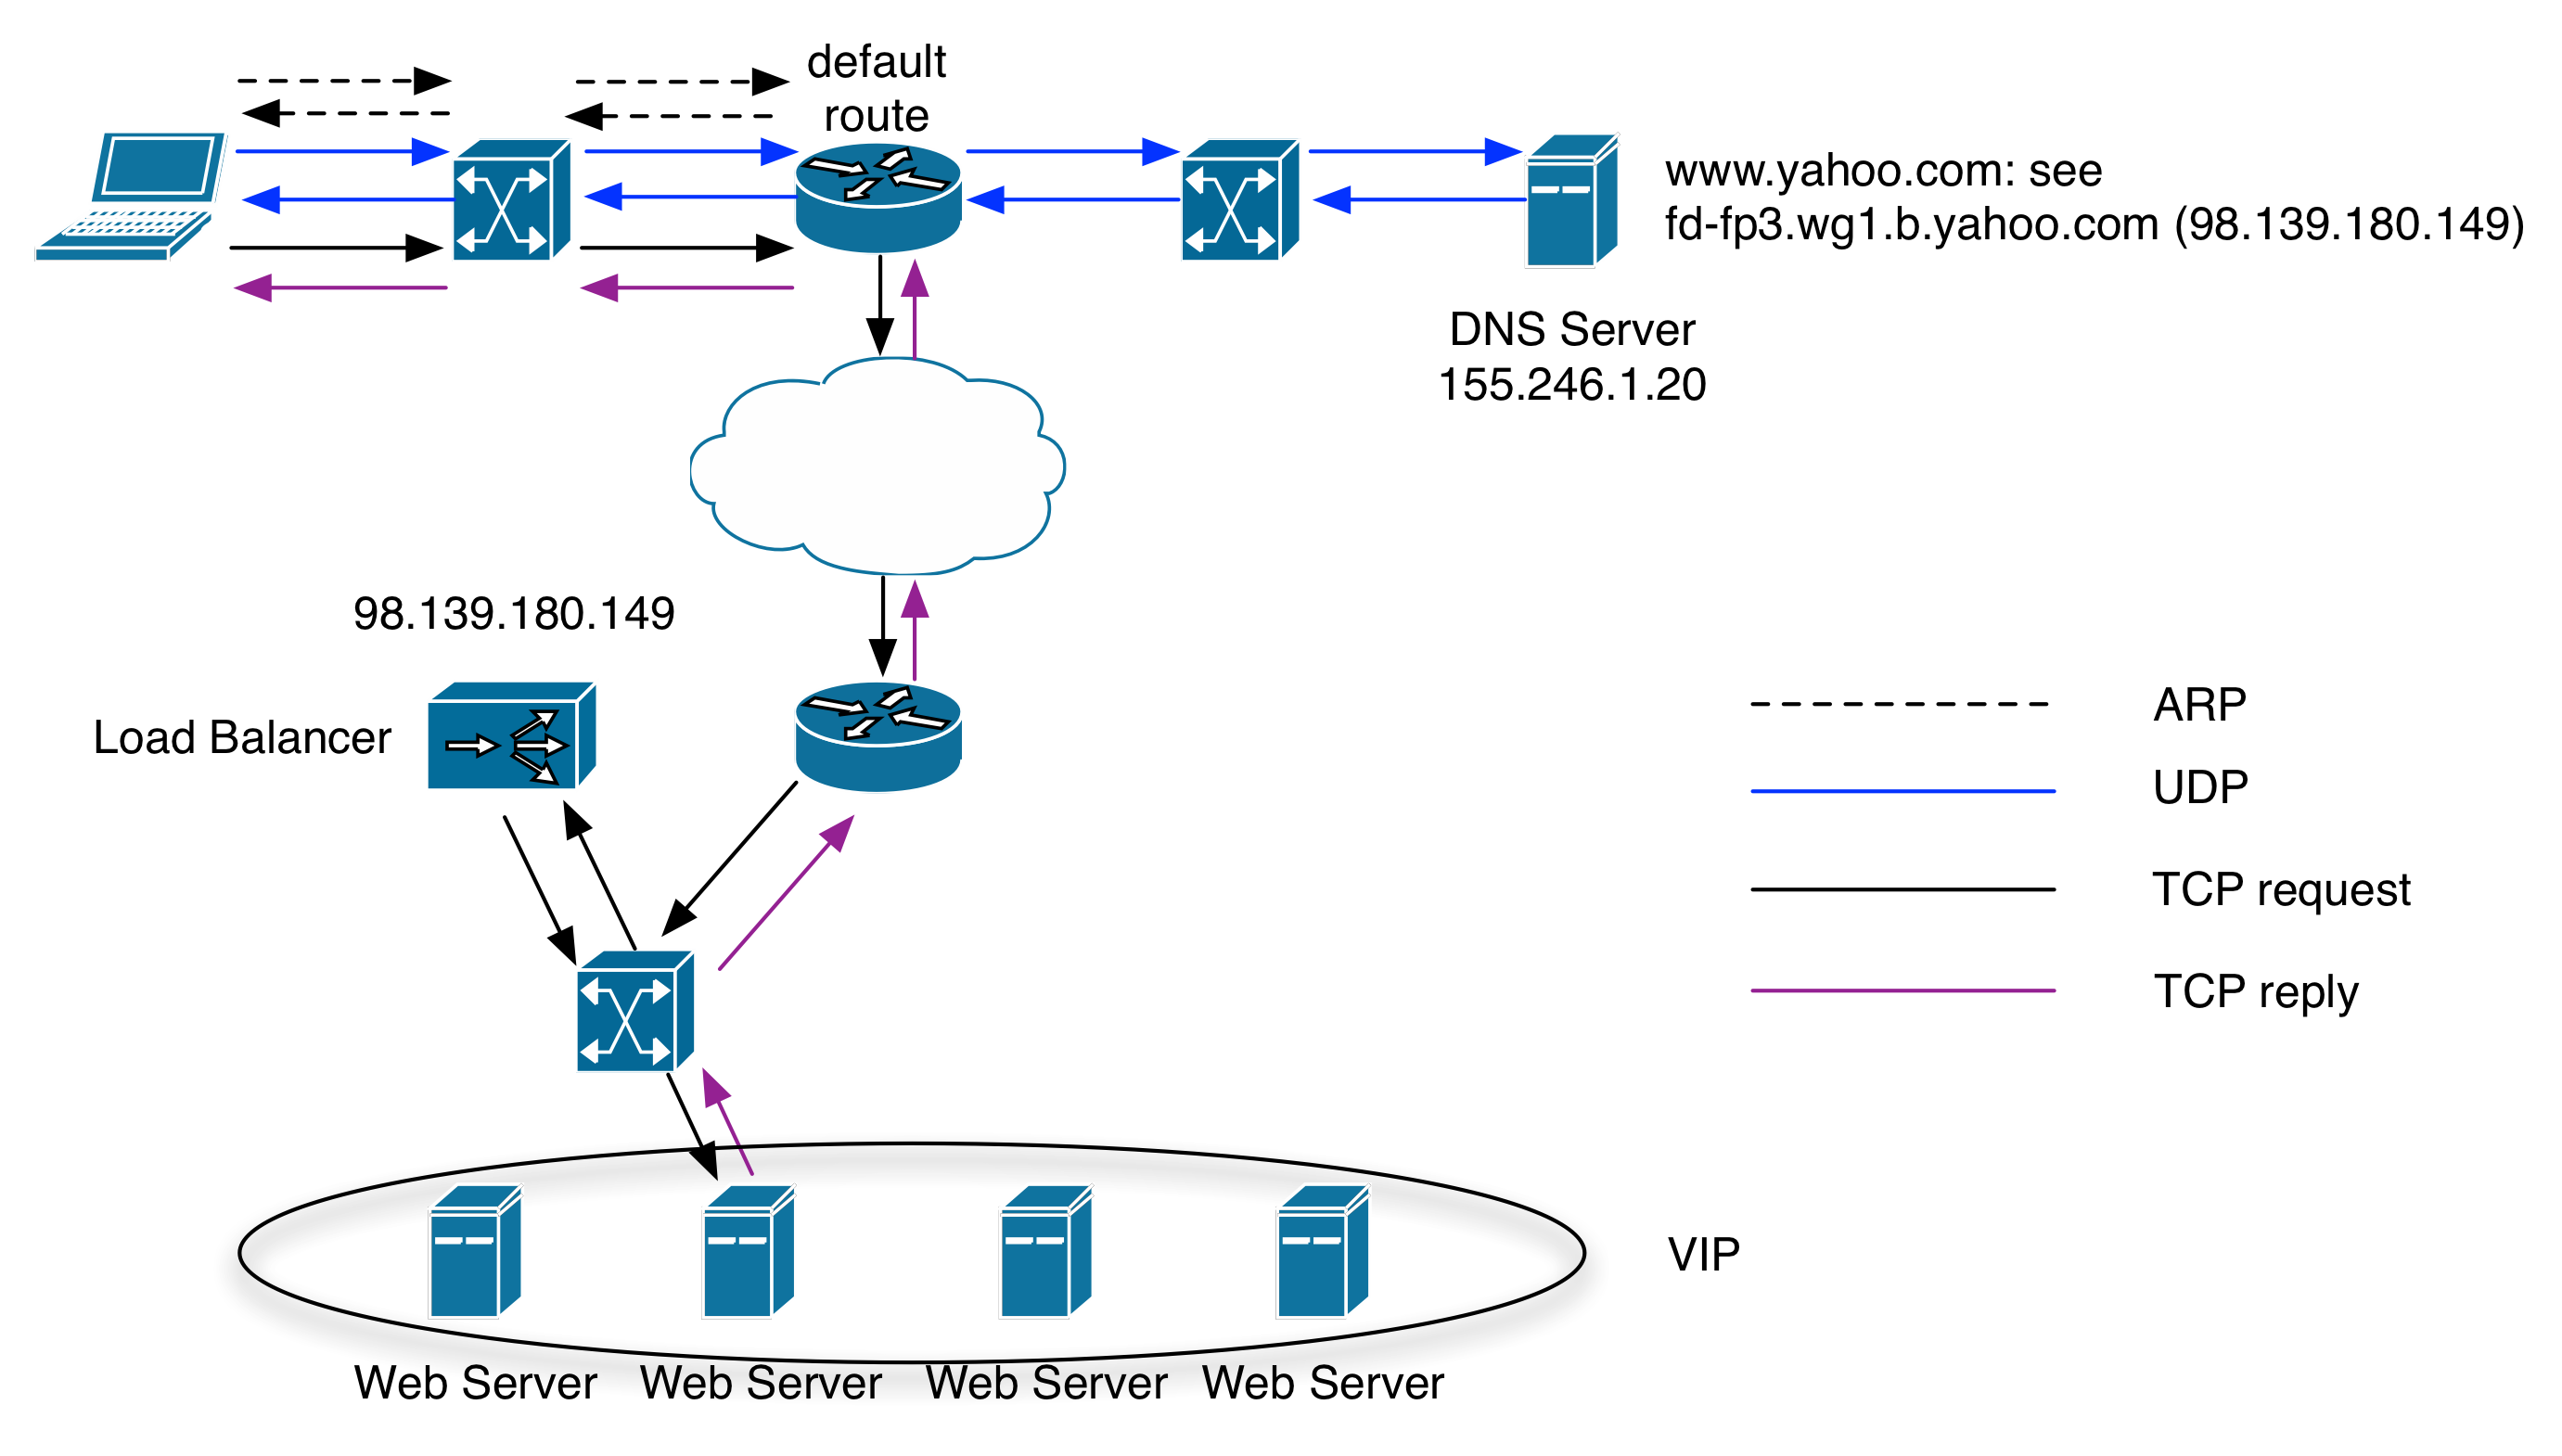
\includegraphics[scale=0.8]{pics/dsr.eps} \\
\end{center}
\vspace*{\fill}

\subsection{TCP/IP Basics: Putting it all together}
\vspace*{\fill}
\begin{center}
	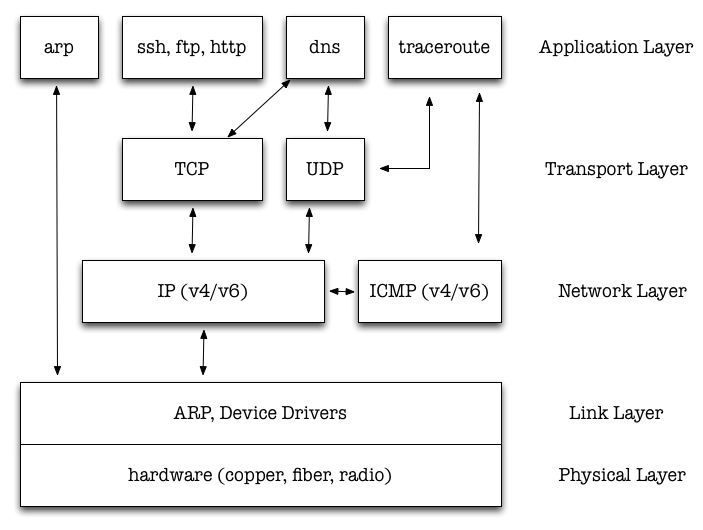
\includegraphics[scale=0.6]{pics/tcpip-stack.eps}
\end{center}
\vspace*{\fill}

\newpage
\vspace*{\fill}
\begin{center}
    \Hugesize
        Lecture 07 \\ [1em]
    \hspace*{5mm}
    \blueline\\
    \hspace*{5mm}\\
	DNS; HTTP
\end{center}
\vspace*{\fill}

\subsection{The New Phonebook is here!}
\vspace*{\fill}
\begin{center}
	\verb+http://is.gd/XXp2sC+ \\
	\addvspace{.5in}
	\verb+wget -q -O - http://is.gd/XXp2sC | grep -c "^HOST"+
\end{center}
\vspace*{\fill}

\subsection{DNS: A hierarchical system}
\vspace*{\fill}
\begin{center}
	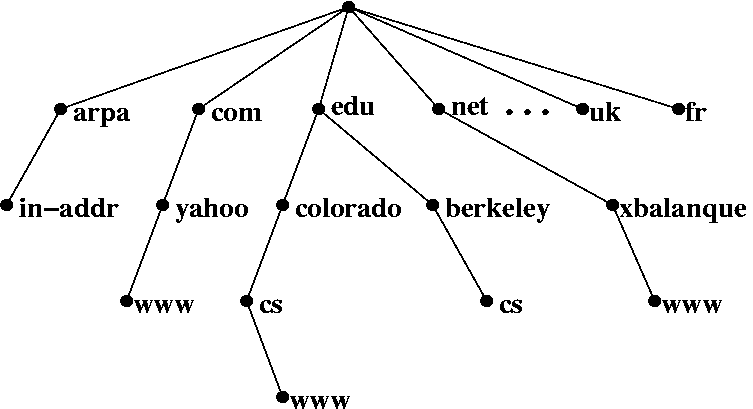
\includegraphics[scale=0.75]{pics/hierarchical-dns.eps}
\end{center}
\vspace*{\fill}

\subsection{Hostname resolution}
\vspace*{\fill}
\begin{center}
	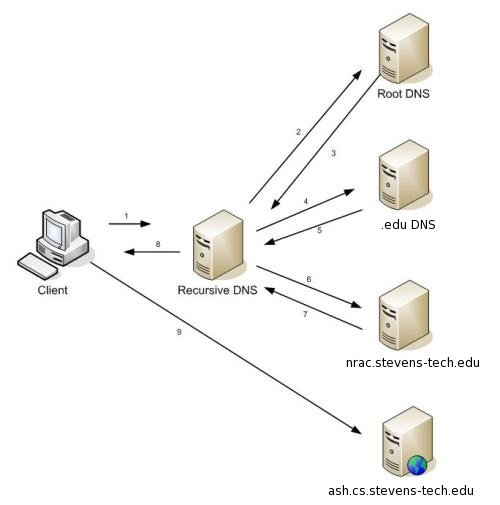
\includegraphics[scale=0.9]{pics/resolution.eps}
\end{center}
\vspace*{\fill}

\subsection{DNS: A distributed database}
\vspace*{\fill}
\begin{center}
	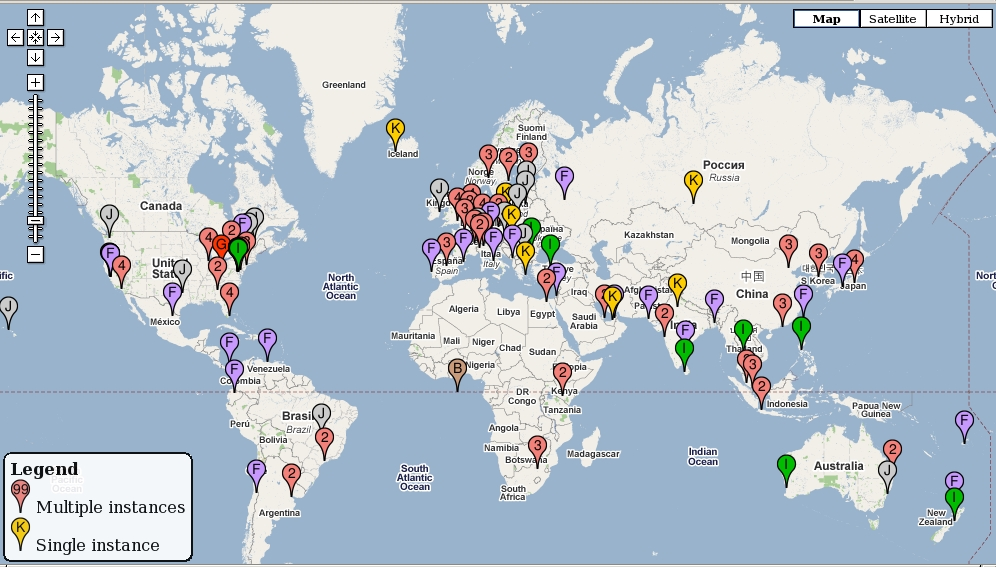
\includegraphics[scale=0.5]{pics/root-servers.eps}
\end{center}
\vspace*{\fill}

\subsection{Creative uses of DNS Resource Records}
\begin{itemize}
	\item identifying sources of SPAM
	\item find out if the internet is on fire: \\
		\verb|dig +short txt istheinternetonfire.com|
	\item find ASN numbers by IP addresses: \\
		\verb|dig +short 159.89.246.155.origin.asn.cymru.com TXT|
	\item check a resolver's source port randomization (to help
		mitigate DNS Cache Poisoning attacks): \\
		\verb|dig +short porttest.dns-oarc.net TXT|
	\item using DNS to publish SSH key fingerprints (RFC4255,
ssh\_config(5) \verb+VerifyHostKeyDNS+; for best results combine with DNSSEC): \\
		\verb|dig +short ftp.netbsd.org SSHFP|
		\begin{verbatim}
ssh -o "VerifyHostKeyDNS yes" ftp.netbsd.org
[...]
Matching host key fingerprint found in DNS.
Are you sure you want to continue connecting (yes/no)?
\end{verbatim}
\end{itemize}

\subsection{The Hypertext Transfer Protocol}
HTTP is a request/response protocol:
\begin{enumerate}
	\item client sends a request to the server
		\begin{itemize}
			\item request method
			\item URI
			\item protocol version
			\item request modifiers
			\item client information
		\end{itemize}
	\item server responds
		\begin{itemize}
			\item status line (including success or error code)
			\item server information
			\item entity metainformation
			\item content
		\end{itemize}
\end{enumerate}

\subsection{HTTP Proxy Servers}
\begin{itemize}
	\item HTTP traffic usually is very asymmetric
	\item a lot of the content is static
	\item network ACLs may restrict traffic flow
\end{itemize}
\vspace{.25in}
\begin{center}
	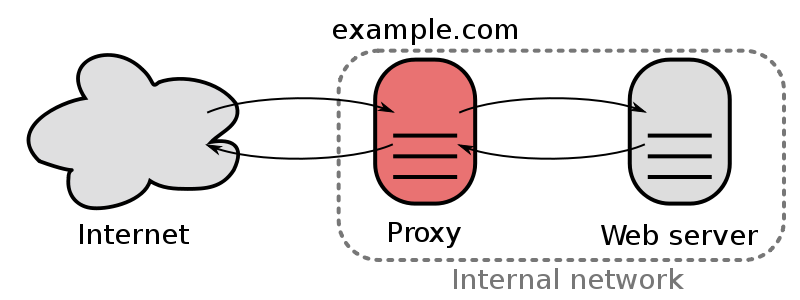
\includegraphics[scale=0.6]{pics/revproxy.eps}
\end{center}

\subsection{Content Delivery Networks}
\begin{itemize}
	\item cache content in strategic locations
	\item determine location to serve from via geomapping of IP
		addresses (beware IPv6 aggregation!)
	\item often uses a separate domain to distinguish small
		objects/large objects or dynamic content/static content
	\item either out-sourced or in-house (if your organization is a
		Tier-1 or Tier-2 peering partner)
	\item request routing happens via Global Server Load Balancing,
		DNS-based request routing, anycasting etc.
	\item provides vast amounts of interesting data about your clients
		(see \verb+http://www.akamai.com/stateoftheinternet/+)
\end{itemize}

\newpage
\vspace*{\fill}
\begin{center}
    \Hugesize
        Lecture 08 \\ [1em]
    \hspace*{5mm}
    \blueline\\
    \hspace*{5mm}\\
	HTTPS; Monitoring
\end{center}
\vspace*{\fill}

\subsection{TLS}
Transport Layer Security
\begin{itemize}
	\item set of cryptographic protocols
	\item operates on layer 6 of OSI stack (Presentation Layer)
	\item independent of HTTP
	\item RFC5246 (TLS 1.2)
\end{itemize}
\addvspace{.5in}
Two distinct security mechanisms:
\begin{enumerate}
	\item encryption of data in transit
	\item authentication of parties
\end{enumerate}

\subsection{TLS}
Protocol:
\begin{itemize}
	\item Client Hello, present list of supported cipher suites
	\item Server Hello, chosen cipher suite
	\item Server Certificate
	\item (Server Key Exchange Message), (Client Certificate Request), (Client Certificate)
	\item Client Key Exchange Message
	\item (Certificate Verify)
	\item (Client Change Cipher Spec), (Server Change Cipher Spec)
\end{itemize}

\subsection{TLS}
\begin{center}
	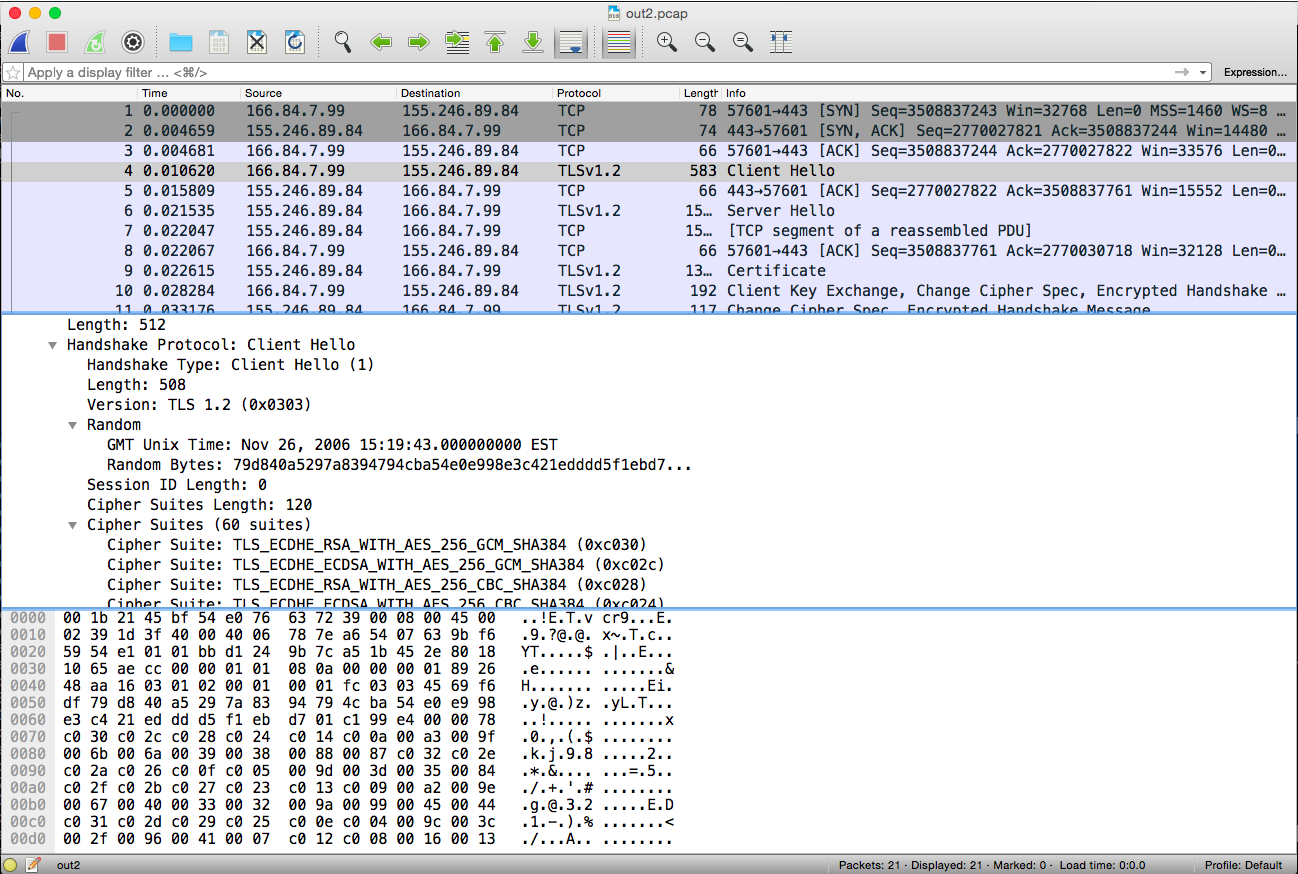
\includegraphics[scale=0.4]{pics/wireshark.eps}
\end{center}

\subsection{TLS}
\begin{verbatim}
$ openssl s_client -connect www.cs.stevens.edu:443
[...]
New, TLSv1/SSLv3, Cipher is DHE-RSA-AES256-SHA
Server public key is 2048 bit
Secure Renegotiation IS supported
Compression: NONE
Expansion: NONE
SSL-Session:
    Protocol  : TLSv1
    Cipher    : DHE-RSA-AES256-SHA
    Session-ID: 5F8A9B7A93EF87009EFCC17BBD68938C56EAACD9DF4C3643EF034D047C9F44C9
    Session-ID-ctx: 
    Master-Key: 20CBA1E477A8B573F29759045329EF7AA38C763C4C41606A46FBCC824C3F32F708789311E7B4275470E35CF09518FDCD
    Key-Arg   : None
    Start Time: 1460395966
    Timeout   : 300 (sec)
    Verify return code: 0 (ok)
\end{verbatim}

\subsection{TLS}
\begin{verbatim}
$ openssl s_client -connect www.cs.stevens.edu:443 | \
        openssl x509 -text -noout
[...]
        Signature Algorithm: sha1WithRSAEncryption
        Issuer: C=US, ST=Arizona, L=Scottsdale, O=GoDaddy.com, Inc., OU=http://certificates.godaddy.com/repository, CN=Go Daddy Secure Certification Authority/serialNumber=07969287
        Validity
            Not Before: Apr 22 13:14:11 2013 GMT
            Not After : Nov  8 15:26:38 2016 GMT
        Subject: OU=Domain Control Validated, CN=www.srcit.stevens.edu
        Subject Public Key Info:
            Public Key Algorithm: rsaEncryption
            RSA Public Key: (2048 bit)
[...]
            X509v3 Subject Alternative Name: 
                DNS:www.srcit.stevens.edu, DNS:srcit.stevens.edu, DNS:svn.srcit.stevens.edu,
                DNS:www.cs.stevens.edu, DNS:guinness.cs.stevens.edu, DNS:rcs.srcit.stevens.edu
\end{verbatim}

\subsection{Requesting a certificate}
\begin{center}
	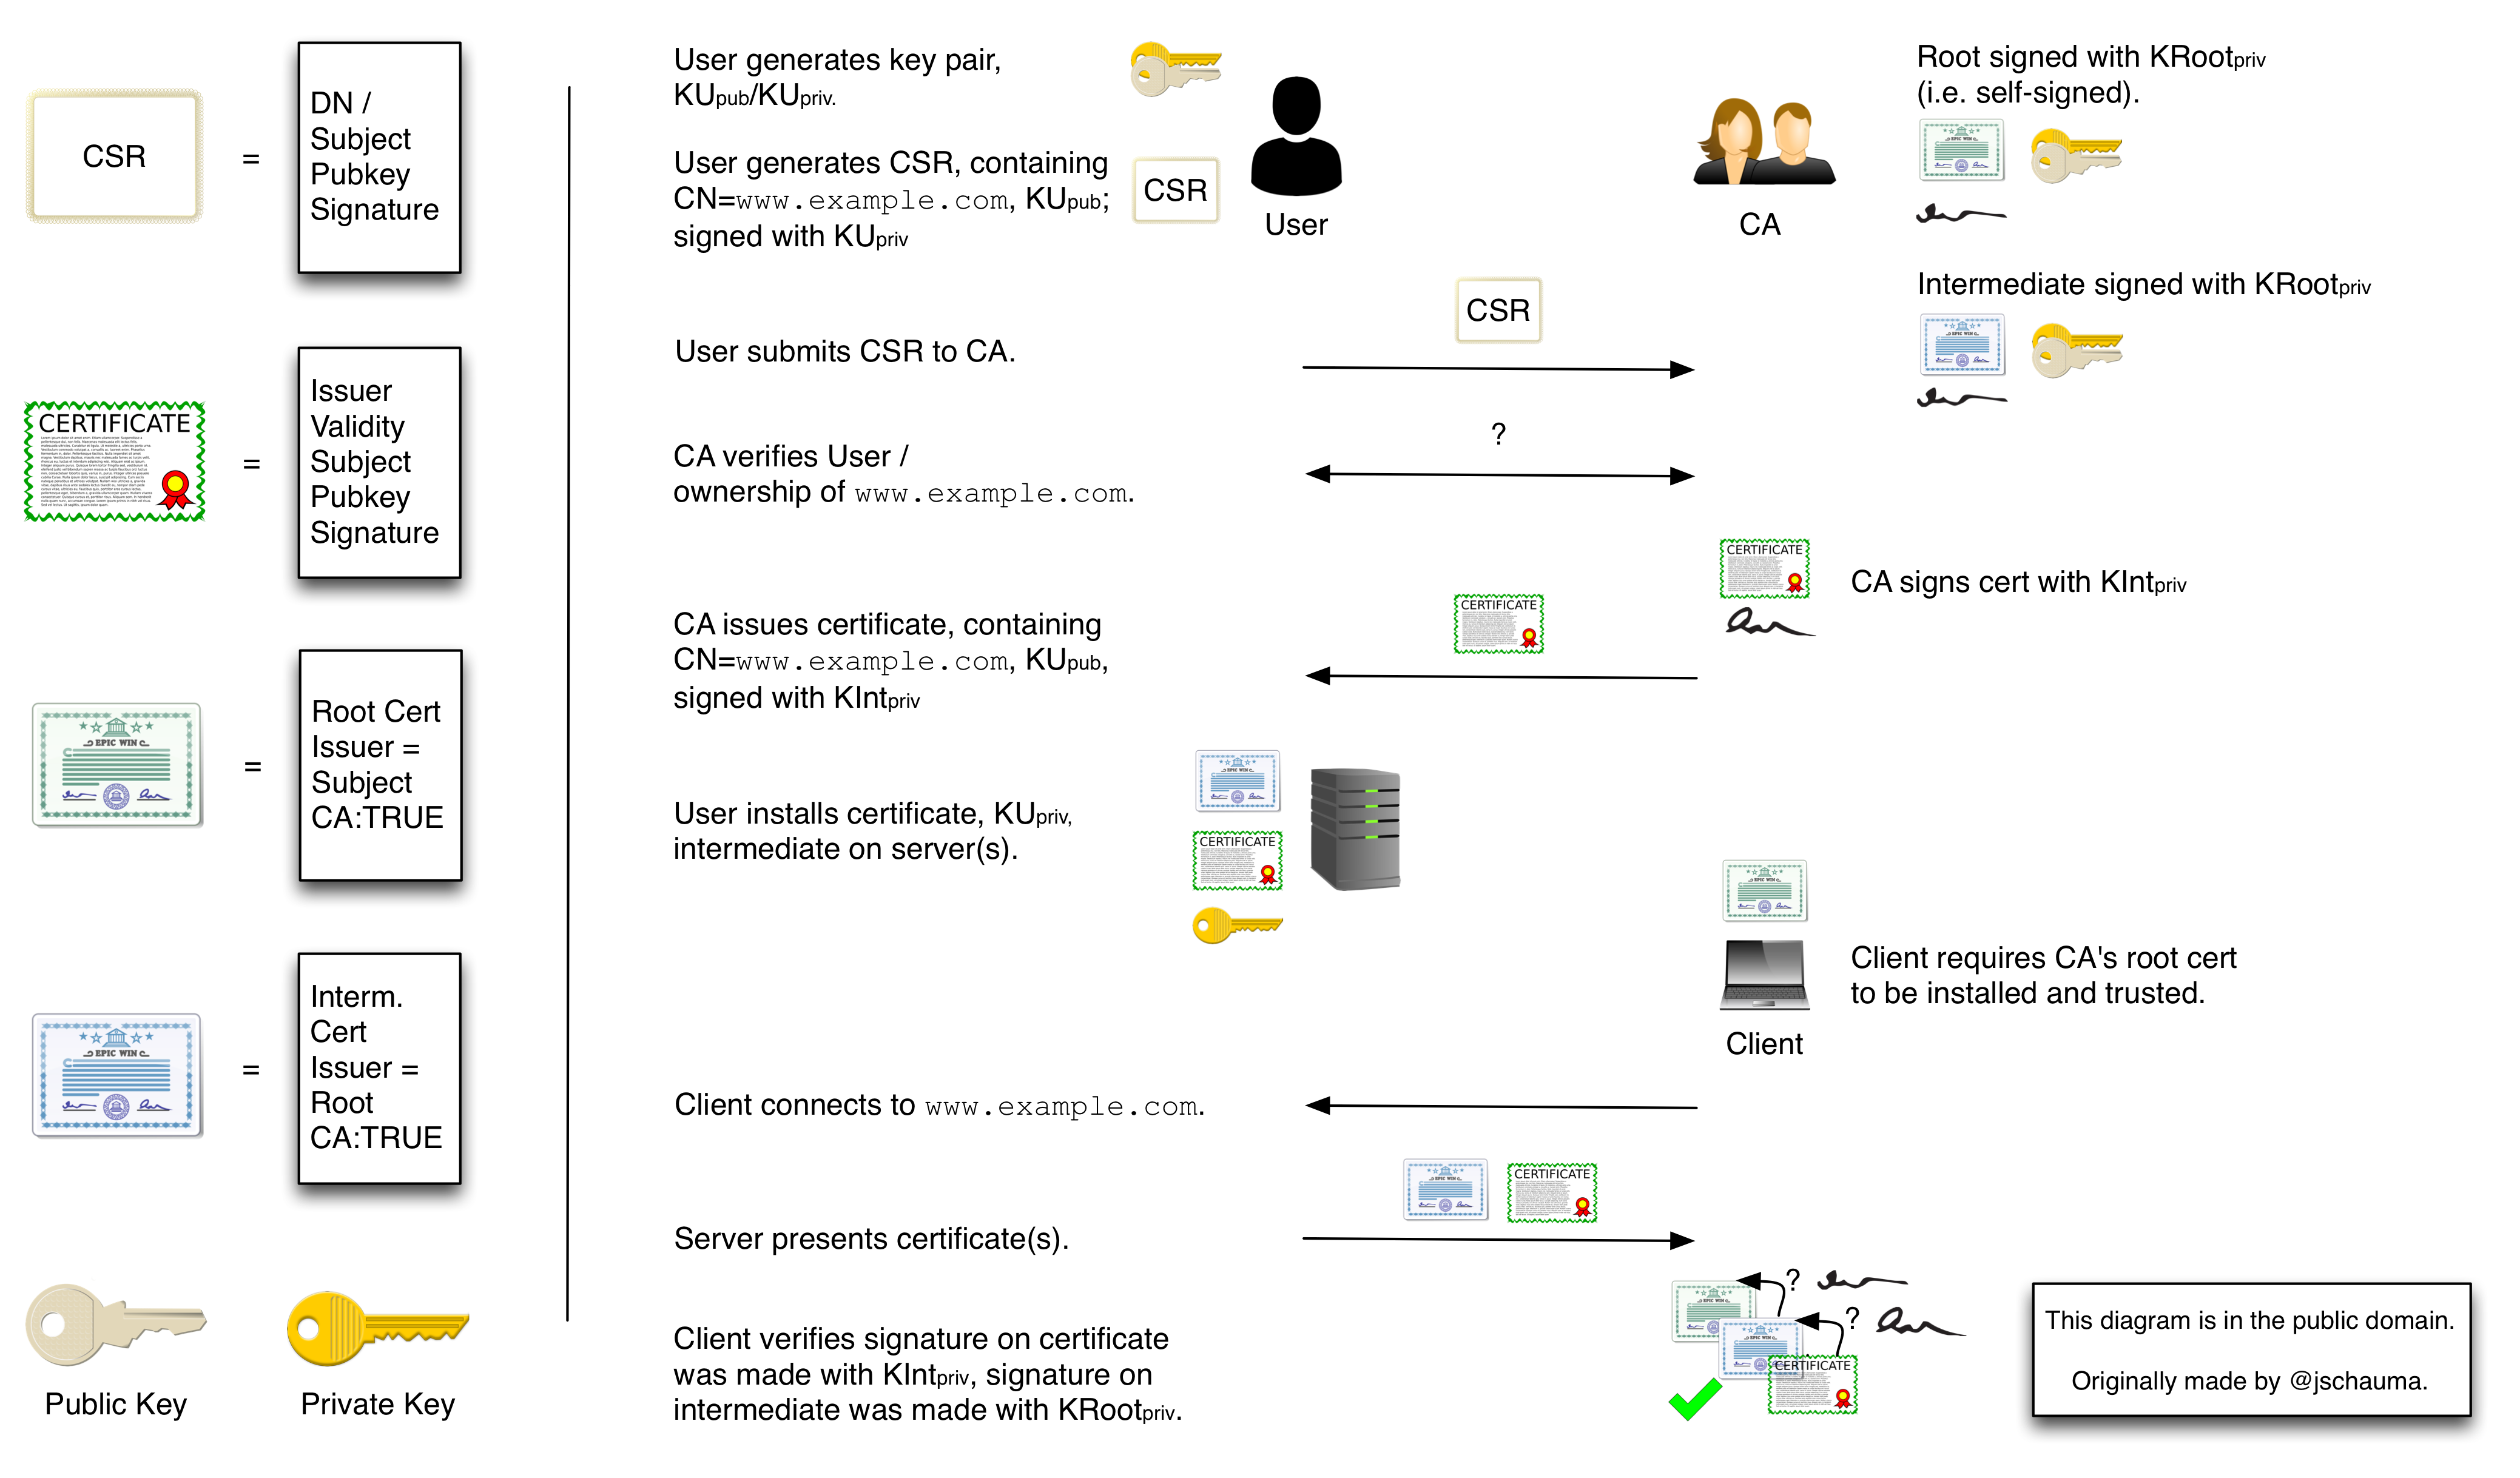
\includegraphics[scale=0.55]{pics/csr-process.eps}
\end{center}

\subsection{TLS Pitfalls}
Lack of universal HTTPS exposes users to significant
risks; many sites don't get the importance of
authentication for non-sensitive content. \\

In order to serve content, you need to have the
private key $ => $ privkey available at perimeter and
exposed, high-risk systems. \\

Rotation/renewal of keys requires routine processes,
which further expose the private key. \\

Control of a CA or a CA's key grants you near
universal powers. \\


\subsection{TLS Pitfalls}
Complex protocols, buggy implementations, intentional
weaknesses and backwards compatibility are just the
high level points.

\begin{itemize}
	\item SSLv2 obsoleted in 1996; 2016: DROWN attack
	\item SSLv3 obsoleted in 1999; 2014: POODLE attack
	\item BEAST, CRIME, BREACH, HEARTBLEED, GotoFail...
	\item obsolete and broken algorithms widely used (RC4, MD5, SHA1, ...)
\end{itemize}

\subsection{Events}
\vspace*{\fill}
\Huge
\begin{center}
``Something's wrong.'' is just an {\em unexpected} or
{\em undesirable} event. \\
\vspace{.4in}
{\em Events} happen all the time. \\
\vspace{.4in}
Being able to identify {\em relevant} events allows
you to diagnose, predict and even prevent {\em
undesirable} events.
\end{center}
\Normalsize
\vspace*{\fill}

\subsection{Events and Metrics}
\vspace*{\fill}
\begin{verbatim}
$ dict event
  event
      n 1: something that happens at a given place and time
      2: a special set of circumstances; "in that event, the first
         possibility is excluded"; "it may rain in which case the
         picnic will be canceled" [syn: {event}, {case}]


$ dict metric
  metric
      3: a system of related measures that facilitates the
         quantification of some particular characteristic [syn:
         {system of measurement}, {metric}]

\end{verbatim}
\vspace*{\fill}

\subsection{Events and Metrics}
\begin{center}
	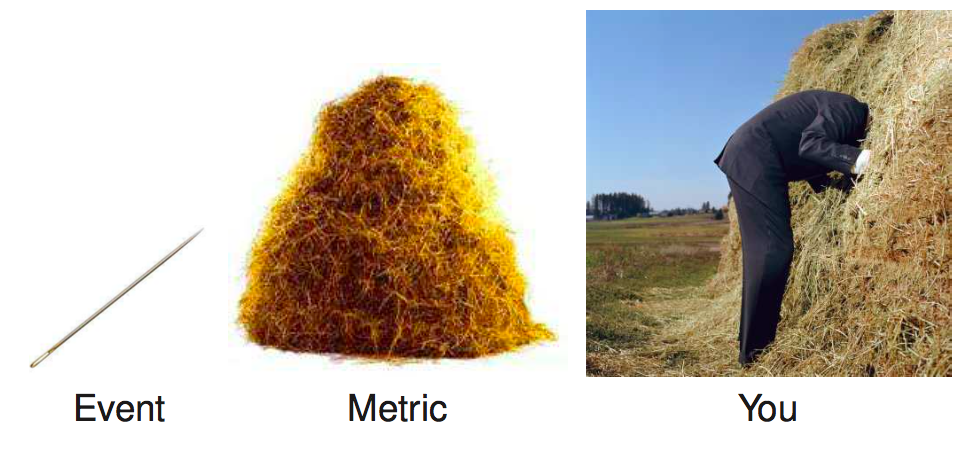
\includegraphics[scale=0.75]{pics/events-metrics.eps}
\end{center}

\subsection{Context}
{\em Context} lets you find {\em relevant} events in
your haystack of metrics.

\begin{center}
	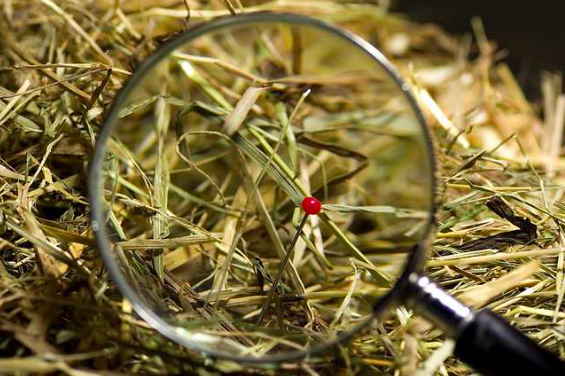
\includegraphics[scale=0.75]{pics/glass-needle.eps}
\end{center}

\subsection{Monitoring Pitfalls}
\vspace*{\fill}
\Huge
\begin{center}
Increasing the size of your haystack does not always
help in finding the needle. \\
\vspace{.4in}
Email is not a scalable network monitoring solution. \\
\vspace{.4in}
Absence of a signal can itself be a signal. \\
\vspace{.4in}
This list is incomplete.
\end{center}
\Normalsize
\vspace*{\fill}

\newpage
\vspace*{\fill}
\begin{center}
    \Hugesize
        Lecture 09 \\ [1em]
    \hspace*{5mm}
    \blueline\\
    \hspace*{5mm}\\
	Writing System Tools
\end{center}
\vspace*{\fill}

\subsection{Tools}
\vspace*{\fill}
\begin{center}
	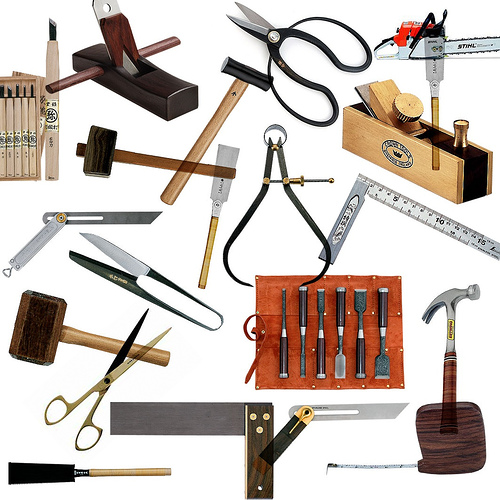
\includegraphics[scale=1.4]{pics/tools.eps}
\end{center}
\vspace*{\fill}

\subsection{Unix Philosophy}
\\
\Huge
\begin{center}
	Write programs that do one thing and do it well.\\
	\vspace{.5in}
	Write programs to work together. \\
	\vspace{.5in}
	Write programs to handle text streams, because that is a universal interface.
\end{center}
\Normalsize

\subsection{Know your languages / eco-system}
Some advice transcends language: \\

\small
\begin{verbatim}
$ echo import this | python
The Zen of Python, by Tim Peters

Beautiful is better than ugly.
Explicit is better than implicit.
Simple is better than complex.
Complex is better than complicated.
Flat is better than nested.
Sparse is better than dense.
Readability counts.
Special cases aren't special enough to break the rules.
Although practicality beats purity.
Errors should never pass silently.
Unless explicitly silenced.
In the face of ambiguity, refuse the temptation to guess.
There should be one-- and preferably only one --obvious way to do it.
Although that way may not be obvious at first unless you're Dutch.
Now is better than never.
Although never is often better than *right* now.
If the implementation is hard to explain, it's a bad idea.
If the implementation is easy to explain, it may be a good idea.
Namespaces are one honking great idea -- let's do more of those!
\end{verbatim}
\Normalsize

\subsection{Learn to write a detailed bug report}
Pre-requisite: Do your homework. \\

Required:
\begin{itemize}
	\item Description Of Problem
	\item Steps To Reproduce
	\item Expected Results
	\item Actual Results
\end{itemize}
\vspace{.125in}

Optional / recommended:
\begin{itemize}
	\item Screenshots / {\em exact} copy of terminal I/O ({\tt script(1)})
	\item Suggested Remediation
	\item Code Patch
\end{itemize}

\subsection{Scalability}
\begin{itemize}
	\item Simplify!
	\item Reduce or eliminate interactions with the user.
	\item Premature optimization is the root of all evil.
	\item So is excusing shoddy programming.
	\item Fix {\em all} warnings and errors.
	\item Document all assumptions.  Be specific.
	\item Always apply the Principle of Least Privilege.
	\item Assume hostile input and usage.
	\item Understand your code.
\end{itemize}


\newpage
\vspace*{\fill}
\begin{center}
    \Hugesize
        Lecture 10 \\ [1em]
    \hspace*{5mm}
    \blueline\\
    \hspace*{5mm}\\
	SMTP; Backup and Disaster Recovery
\end{center}
\vspace*{\fill}

\subsection{Sending...}
\begin{verbatim}
# tcpdump -i xennet0 -w /tmp/t.out port not 22 2>/dev/null &
# mail -s "CS615 - SMTP Exercise" jschauma@stevens.edu -f jschauma@stevens.edu
Hello,

SMTP is simple.

-Jan
.
EOT
# fg
tcpdump -i xennet0 -w /tmp/t.out port not 22 2>/dev/null
^C
\end{verbatim}


\subsection{Sending...}
\begin{verbatim}
# tail -5 /var/log/maillog
Apr  4 15:42:33 ip-10-235-167-232 postfix/pickup[848]: 2A17275438:
        uid=0 from=<jschauma@stevens.edu>
Apr  4 15:42:33 ip-10-235-167-232 postfix/cleanup[765]: 2A17275438:
        message-id=<20160404154233.2A17275438@ip-10-235-167-232.ec2.internal>
Apr  4 15:42:33 ip-10-235-167-232 postfix/qmgr[876]: 2A17275438:
        from=<jschauma@stevens.edu>, size=380, nrcpt=1 (queue active)
Apr  4 15:42:33 ip-10-235-167-232 postfix/smtp[1124]: 2A17275438:
        to=<jschauma@stevens.edu>, relay=spamfilter01.stevens.edu[155.246.14.37]:25,
        delay=0.62, delays=0.04/0.01/0.03/0.54, dsn=2.0.0,
        status=sent (250 Ok: queued as 688CD6F4001)
Apr  4 15:42:33 ip-10-235-167-232 postfix/qmgr[876]: 2A17275438: removed
\end{verbatim}

\subsection{Sending...}
\begin{verbatim}
# tcpdump -t -r /tmp/t.out port 53
IP 10.235.167.232.65498 > 172.16.0.23.domain: 61195+ MX? stevens.edu. (29)
IP 172.16.0.23.domain > 10.235.167.232.65498: 61195 2/0/0
        MX spamfilter01.stevens.edu. 10,
        MX spamfilter02.stevens.edu. 20 (87)
IP 10.235.167.232.65497 > 172.16.0.23.domain: 1949+
        A? spamfilter01.stevens.edu. (42)
IP 172.16.0.23.domain > 10.235.167.232.65497: 1949 1/0/0 A 155.246.14.37 (58)
IP 10.235.167.232.65496 > 172.16.0.23.domain: 39922+
        AAAA? spamfilter01.stevens.edu. (42)
IP 172.16.0.23.domain > 10.235.167.232.65496: 39922 0/1/0 (113)
IP 10.235.167.232.65495 > 172.16.0.23.domain: 26844+
        A? spamfilter02.stevens.edu. (42)
IP 172.16.0.23.domain > 10.235.167.232.65495: 26844 1/0/0 A 155.246.248.24 (58)
IP 10.235.167.232.65494 > 172.16.0.23.domain: 1439+
        AAAA? spamfilter02.stevens.edu. (42)
IP 172.16.0.23.domain > 10.235.167.232.65494: 1439 0/1/0 (113)
\end{verbatim}

\subsection{Sending...}
\begin{verbatim}
# host -t mx stevens.edu
stevens.edu mail is handled by 20 spamfilter02.stevens.edu.
stevens.edu mail is handled by 10 spamfilter01.stevens.edu.
# host spamfilter01.stevens.edu.
spamfilter01.stevens.edu has address 155.246.14.37
# host spamfilter02.stevens.edu.
spamfilter02.stevens.edu has address 155.246.248.24
#
\end{verbatim}

\subsection{Sending...}
\begin{Verbatim}
$ telnet 155.246.14.37 25
Trying 155.246.14.37...
Connected to spamfilter01.stevens.edu.
Escape character is '^]'.
\textbf{220 spamfilter01.stevens.edu ESMTP (fe32969a29a5f461e53bf93b18c8fdb5)}
EHLO ip-10-235-167-232.ec2.internal
\textbf{250-spamfilter01.stevens.edu Hello ec2-54-205-68-41.compute-1.amazonaws.com [54.205.68.41],}
\textbf{        pleased to meet you}
\textbf{250-SIZE 50000000}
\textbf{250-PIPELINING}
\textbf{250-8BITMIME}
\textbf{250 HELP}
MAIL FROM:<jschauma@stevens.edu> SIZE=380
\textbf{250 Sender <jschauma@stevens.edu> OK}
RCPT TO:<jschauma@stevens.edu>
\textbf{250 Recipient <jschauma@stevens.edu> OK}
\end{Verbatim}

\subsection{Sending...}
\begin{Verbatim}
DATA
\textbf{354 Start mail input; end with <CRLF>.<CRLF>}
Received: by ip-10-235-167-232.ec2.internal (Postfix, from userid 0)
        id 2A17275438; Mon,  4 Apr 2016 15:42:33 +0000 (UTC)
To: jschauma@stevens.edu
Subject: CS615 - SMTP Exercise
Message-Id: <20160404154233.2A17275438@ip-10-235-167-232.ec2.internal>
Date: Mon,  4 Apr 2016 15:42:33 +0000 (UTC)
From: jschauma@stevens.edu (Charlie Root)

Hello,

SMTP is simple.

-Jan
.
\textbf{250 Ok: queued as 6A9C76F4004}
\end{Verbatim}

\subsection{Receiving...}
\smallish
\begin{verbatim}
From jschauma@stevens.edu  Mon Apr  4 11:42:35 2016
Received: by panix.netmeister.org (Postfix, from userid 1004)
        id 6B0F56513D; Mon,  4 Apr 2016 11:42:35 -0400 (EDT)
Received: from nexus.stevens.edu (nexus.stevens.edu [155.246.14.12])
        by panix.netmeister.org (Postfix) with ESMTP id 2AD596513B
Received: from exchng02.campus.stevens-tech.edu (exchng02.campus.stevens-tech.edu [155.246.14.23])
        by nexus.stevens.edu (Postfix) with ESMTPS id 11E3817F825
Received: from exchng04.campus.stevens-tech.edu (2002:9bf6:f826::9bf6:f826) by
        exchng02.campus.stevens-tech.edu (2002:9bf6:e17::9bf6:e17) with Microsoft
        SMTP Server (TLS) id 15.0.1104.5; Mon, 4 Apr 2016 11:42:34 -0400
Received: from exchng03.campus.stevens-tech.edu (155.246.248.36) by
        exchng04.campus.stevens-tech.edu (155.246.248.39) with Microsoft SMTP Server
        (TLS) id 15.0.1104.5; Mon, 4 Apr 2016 11:42:34 -0400
Received: from exchng03.campus.stevens-tech.edu ([::1]) by
        exchng03.campus.stevens-tech.edu ([fe80::599a:f128:d1b3:4ce7%12]) with
        Microsoft SMTP Server id 15.00.1104.000; Mon, 4 Apr 2016 11:42:34 -0400
From: Jan Schaumann <jschauma@stevens.edu>
To: Jan Schaumann <jschauma@stevens.edu>
Subject: CS615 - SMTP Exercise
Date: Mon, 4 Apr 2016 15:42:33 +0000
Message-ID: <1b1399e9c44b494f99e9d0030f0fa74b@exchng03.campus.stevens-tech.edu>
x-barracuda-apparent-source-ip: 54.205.68.41
x-ms-exchange-parent-message-id: <20160404154233.2A17275438@ip-10-235-167-232.ec2.internal>
Resent-Message-Id: <20160404154235.11E3817F825@nexus.stevens.edu>
\end{verbatim}

\subsection{Receiving...}
\begin{verbatim}
$ tail -f /var/log/maillog
postfix/smtpd[552]: connect from nexus.stevens.edu[155.246.14.12]
postfix/smtpd[552]: 2AD596513B: client=nexus.stevens.edu[155.246.14.12]
postfix/cleanup[6975]: 2AD596513B:
        message-id=<1b1399e9c44b494f99e9d0030f0fa74b@exchng03.campus.stevens-tech.edu>
postfix/cleanup[6975]: 2AD596513B:
        resent-message-id=<20160404154235.11E3817F825@nexus.stevens.edu>
postfix/smtpd[552]: disconnect from nexus.stevens.edu[155.246.14.12]
postfix/qmgr[24644]: 2AD596513B: from=<jschauma@stevens.edu>, size=3116, nrcpt=1 (queue active)
spamd[24829]: spamd: connection from localhost [::1]:58531 to port 783, fd 5
spamd: processing message <1b1399e9c44b494f99e9d0030f0fa74b@exchng03.campus.stevens-tech.edu>
        aka <20160404154235.11E3817F825@nexus.stevens.edu> for spamd:1004
postfix/pipe[8278]: 2AD596513B: to=<jschauma@netmeister.org>, relay=spamassassin, delay=0.29,
        delays=0.05/0.01/0/0.23, dsn=2.0.0, status=sent (delivered via spamassassin service)
postfix/qmgr[24644]: 2AD596513B: removed
postfix/pickup[16387]: 6B0F56513D: uid=1004 from=<jschauma@stevens.edu>
postfix/cleanup[6975]: 6B0F56513D:
        message-id=<1b1399e9c44b494f99e9d0030f0fa74b@exchng03.campus.stevens-tech.edu>
postfix/cleanup[6975]: 6B0F56513D:
        resent-message-id=<20160404154235.11E3817F825@nexus.stevens.edu>
postfix/qmgr[24644]: 6B0F56513D: from=<jschauma@stevens.edu>, size= 3442, nrcpt=1 (queue active)
postfix/local[2264]: 6B0F56513D: to=<jschauma@netmeister.org>, relay=local,
        delay=0.15, delays=0.08/0.01/0/0.06, dsn=2.0.0, status=sent (delivered to command:
        /usr/pkg/bin/procmail)
\end{verbatim}
\Normalsize

\subsection{SMTP is a Simple Mail Transfer Protocol.}

\begin{itemize}
	\item TCP port 25
	\item DNS MX records
	\item mail may be relayed or processed by many servers in transit
	\item transport is in clear text
	\item STARTTLS may provide (opportunistic) transport encryption
	\item SPAM controls may include DNS lookups, bayesian scoring, ...
	\item authenticity not guaranteed
\end{itemize}

\subsection{The Mail System}
Divided into:
\begin{itemize}
	\item {\em Mail User Agent} or MUA, such as {\tt mutt(1)}, {\em Mail.app}, {\em Outlook}, a browser (ugh) ...
	\item {\em Mail Transfer Agent} or MTA, such as {\em postfix},
		{\em sendmail}, {\em qmail}, ...
	\item {\em Mail Delivery Agent} or MDA, such as {\em procmail}
	\item {\em Access Agent} providing access via {\em POP}, {\em IMAP} etc.
\end{itemize}

\subsection{Anatomy of an email message}
An email consists of:
\begin{itemize}
	\item mandatory headers (such as "From ", "Delivered-To: ", ...)
	\item optional headers (such as "From: ", "To: ", "Subject: ", ...)
	\item the (optional) body of the message
\end{itemize}

\subsection{Service Considerations}
\begin{itemize}
	\item outsourcing versus in-house
	\item privacy considerations
	\item spam protections
	\item phishing protections
	\item mail delivery cannons for notifications vs. spam lists
	\item high volume traffic demands fine-tuned systems
	\item high volume traffic implications on logging
\end{itemize}
\vspace{.5in}
See also:
\begin{itemize}
	\item {\tt http://is.gd/JQp1zM}
	\item {\tt http://is.gd/cXyrwX}
	\item {\tt http://is.gd/o6Y5f8}
\end{itemize}

\subsection{Backups and Restore Basics}
When do we need backups?
\begin{itemize}
	\item disaster recovery: off-site storage of sensitive data
	\item long-term storage requirements
	\item recover from data loss due to
		\begin{itemize}
			\item equipment failure
			\item bozotic users
			\item natural disaster
			\item security breach
			\item software bugs
		\end{itemize}
\end{itemize}
\addvspace{.5in}
Think of your backups as {\em insurance}:  you invest and pay for it, hoping
you will never need it.

\subsection{Filesystem backup}
Example: WAFL (Write Anywhere File Layout)
\vspace*{\fill}
\begin{center}
	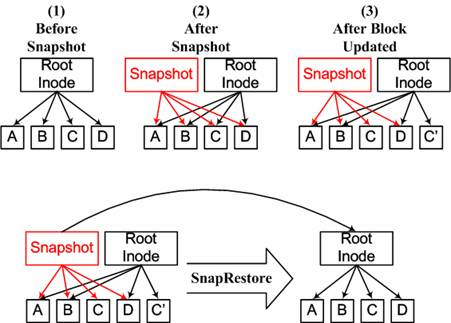
\includegraphics[scale=1.0]{pics/wafl.eps}
\end{center}
\vspace*{\fill}

\subsection{Summary}
\begin{itemize}
	\item backups are most commonly done as incrementals
		of a filesystem, mountpoint, or directory hierarchy
	\item consider (long-term) storage:
		\begin{itemize}
			\item media and location
			\item increased storage requirements
			\item privacy and safety of the data
		\end{itemize}
	\item self-service restores and filesystem snapshots
	\item backups need to be:
		\begin{itemize}
			\item regular, frequent, automated
			\item invisible
			\item verifiable
		\end{itemize}
\end{itemize}

\subsection{Summary}
\vspace*{\fill}
\begin{center}
	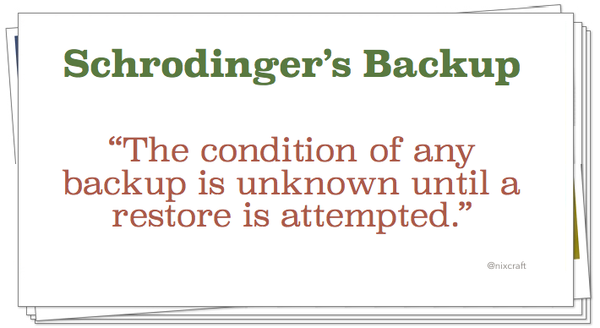
\includegraphics[scale=0.8]{pics/schrodinger.eps}
\end{center}
\vspace*{\fill}



\newpage
\vspace*{\fill}
\begin{center}
    \Hugesize
        Lecture 11 \\ [1em]
    \hspace*{5mm}
    \blueline\\
    \hspace*{5mm}\\
	Configuration Management
\end{center}
\vspace*{\fill}

\subsection{Pets vs. Cattle}
``Pets'':
\begin{itemize}
	\item unique, cheerful hostnames
	\item single systems grown over time, lovingly configured by hand
	\item when sick, everybody is very concerned
	\item slowly nursed back to life
\end{itemize}
\vspace{.25in}
``Cattle'':
\begin{itemize}
	\item predictable, boring hostnames
	\item almost identical to all others
	\item centrally managed, easy to recreate
	\item when sick, they get taken out back and shot
	\item quickly replaced by another
\end{itemize}

\subsection{CM States}
\vspace*{\fill}
\begin{center}
	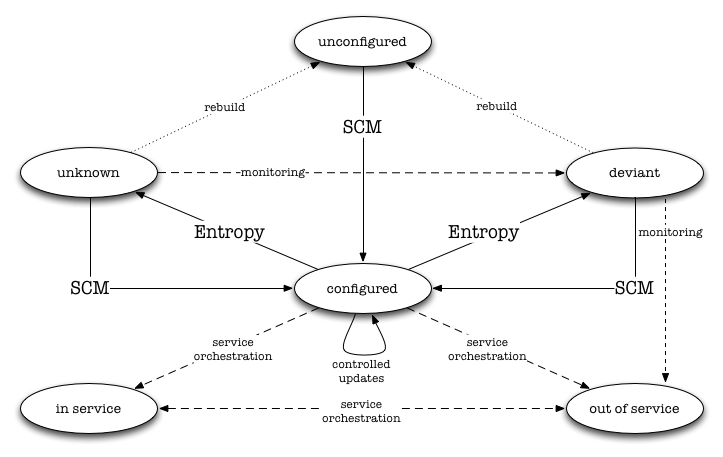
\includegraphics[scale=0.7]{pics/host-states.eps} \\
\end{center}
\vspace*{\fill}

\subsection{Idempotence}
CM systems assert state.  For this, all operations
must be {\em idempotent}. \\
\vspace{.5in}

\begin{displaymath}
f(f(x)) \equiv f(x)
\end{displaymath}

\begin{displaymath}
| |-1| | \equiv |-1|
\end{displaymath}

\begin{verbatim}
$ cd etc                                            # not idempotent
$ rm resolv.conf                                    # idempotent
$ echo "nameserver 192.168.0.1" > resolv.conf       # idempotent
$ echo "nameserver 192.168.0.2" >> resolv.conf      # not idempotent
$ chown root:wheel resolv.conf                      # idempotent
$ chmod 0644 resolv.conf                            # idempotent
\end{verbatim}

\subsection{Convergence and Eventual Consistency}
Note: idempotence does not guarantee efficiency! \\
\vspace{.5in}

CM systems should ensure changes are:
\begin{enumerate}
	\item idempotent (well, that part's on you)
	\item only applied if needed
	\item eventually consistent
\end{enumerate}
\vspace{.5in}

This often requires complexity (oh no!), coordination
with and awareness of other systems.  {\em Service
Orchestration} has developed as a separate, related
discipline to help address this.

\subsection{Distributed Systems}
CM systems are {\em distributed} systems.  As such,
they are subject to the CAP Theorem: \\

{\em Consistency}: all systems managed by the CM are
consistent within their respective service definition.
\\

{\em Availability}: the services managed by the CM are
kept available, even if no further updates or change
sets can be retrieved. \\

{\em Partition tolerance}: the CM system can (continue
to) operate despite interruptions between its
components; e.g. intermediate (coordinated) changes
are not required.

\newpage
\vspace*{\fill}
\begin{center}
    \Hugesize
        Lecture 12 \\ [1em]
    \hspace*{5mm}
    \blueline\\
    \hspace*{5mm}\\
	Ethics and Social Responsibility
\end{center}
\vspace*{\fill}

\subsection{sudo(8)}
\vspace*{\fill}
\begin{verbatim}
We trust you have received the usual lecture from the local System
Administrator. It usually boils down to these three things:
#1) Respect the privacy of others.
#2) Think before you type.
#3) With great power comes great responsibility.
\end{verbatim}
\vspace*{\fill}

\subsection{A Code of Ethics in Internet Operations}
\Huge
\vspace*{\fill}
\begin{center}

We are stewards of our users' data. \\

We are obligated to act in the public interest.

\end{center}
\vspace*{\fill}
\Normalsize

\subsection{Ethics}
The LISA Code of Ethics:
\\

\newcolumntype{S}{>{\centering\arraybackslash} m{.4\linewidth} }
\begin{tabular}{ p{10cm} S }
\begin{itemize}
	\item Professionalism
	\item Personal Integrity
	\item Privacy
	\item Laws and Policies
	\item System Integrity
	\item Education
	\item Social Responsibility
	\item Ethical Responsibility
\end{itemize}
& \multirow{20}{*}{
\includegraphics[scale=1.3]{pics/angel.eps}} \\
\end{tabular}

\subsection{LISA Code of Ethics}
Professionalism and Personal Integrity:

\begin{itemize}
	\item maintain professional conduct; don't let
personal feelings or beliefs interfere
	\item know your competence, know when to seek help
	\item own your mistakes
	\item disclose and recuse yourself under conflicts of interest
\end{itemize}
\vspace{.5in}
Lead by example.


\subsection{LISA Code of Ethics}
Privacy:
\begin{itemize}
	\item only access private information when necessary
	\item protect confidentiality of accidentally learned information
	\item work in teams/pairs
	\item delete, encrypt, anonymize
	\item even better: do not collect the information to begin with
\end{itemize}
\vspace{.5in}
Data is a liability.

\subsection{LISA Code of Ethics}
Laws and Policies:
\begin{itemize}
	\item educate yourself and others on relevant laws, regulations, policies
	\item (work to) elect informed representatives
	\item participate in design and architecture of e.g. technical standards
	\item understand the difference between {\em
legal} and {\em ethical}; between the letter of a law
and the spirit or objective
\end{itemize}
\vspace{.5in}
All politics is local.

\subsection{LISA Code of Ethics}
Communication:
\begin{itemize}
	\item communicate clearly, openly with your users, management, colleagues
	\item listen to the needs of others
	\item document your policies with reason and rationale
\end{itemize}
\vspace{.5in}
``Sunlight is the Best Disinfectant''


\subsection{LISA Code of Ethics}
Education and Community:
\begin{itemize}
	\item continously educate yourself, enhance your technical knowledge
	\item share your knowledge, teach others
	\item attending conferences is not optional
	\item eventually, neither is speaking at conferences
	\item publish your results, research
	\item build ties with peers at other organizations
	\item partake in Open Source, meetups, mailing lists, community events
\end{itemize}
\vspace{.5in}
You are shaped by the community and culture you choose.

\subsection{SysAdmin realities}
\begin{itemize}
	\item you are in a {\em privileged} position
	\item you {\em are} a target
	\item you are {\em obligated} to act in your users' interest
	\item you {\em will} face tough choices
	\item there is {\em no rulebook} to help you decide
	\item the slippery slope is not always steep
	\item you {\em can} make a difference
\end{itemize}

\newpage
\vspace*{\fill}
\begin{center}
    \Hugesize
        Lecture 13 \\ [1em]
    \hspace*{5mm}
    \blueline\\
    \hspace*{5mm}\\
	System Security
\end{center}
\vspace*{\fill}

\subsection{How to determine {\em risk}}
``Risk Assessment''
\begin{itemize}
	\item identify {\em assets}
	\item identify {\em threats}
	\item identify {\em vulnerabilities}
	\item determine {\em likelihood of damage}
	\item estimate {\em cost of recovery}
	\item estimate {\em cost of defense}
\end{itemize}
\vspace{.5in}

A {\em risk} is the {\em likelihood} of a {\em threat} successfully exploiting
a {\em vulnerability} and the {\em estimated cost} (or potential damage) both
in the short and long term you may incur as a result.

\subsection{Threat Model}
For each system/component/product/service/...

\begin{itemize}
	\item identify {\em what} you're protecting
	\item identify {\em whom} you're protecting it {\em from}
		\begin{itemize}
			\item identify {\em goals} of the attacker
			\item identify {\em motivation} of the attacker
			\item identify {\em capabilities} of the attacker
		\end{itemize}
	\item identify threats you cannot defend against (within this
		system or in general)
\end{itemize}

\subsection{Cryptography}
Note:
\begin{itemize}
	\item {\em Authentication} \verb+!=+ {\em Authorization}
	\item cryptography does not handle authorization
	\item you generally need all three: confidentiality, integrity, authenticity
	\item cryptography cannot prevent against incorrect use \\
		(usability is hard, let's go shopping)
\end{itemize}
\addvspace{.5in}
Know your threat model!

\subsection{Secure by default}
\vspace{.5in}
\Huge
\begin{center}
Users care about usability, not about security. \\
\addvspace{.5in}
Users will not change their default settings. \\
\Normalsize
(Unless a less secure option is available.)
\end{center}

\subsection{Embrace Automation}
\vspace*{\fill}
\Huge
\begin{center}
	Vulnerabilities are dense. \\
\addvspace{.5in}
	Eliminate {\em classes} of attacks, not
	individual flaws. \\
\end{center}
\Normalsize
\vspace*{\fill}

\subsection{Build Robust Infrastructures and Service}
\vspace*{\fill}
\Huge
\begin{center}
	Your endpoint security model should assume the
	network is compromised; \\
	your network security model should assume the
	endpoint is. \\
\addvspace{.5in}
	Both in fact are.
\end{center}
\Normalsize
\vspace*{\fill}

\subsection{Threat Model}
\vspace*{\fill}
\Huge
\begin{center}
Your adversaries are determined human actors with
specific goals. \\
\addvspace{.5in}

Constantly seek to reduce your attack surface. \\
Identify and eliminate attack vectors.\\
\addvspace{.5in}

Don't be lazy.
\end{center}
\Normalsize
\vspace*{\fill}

\subsection{This Whole Semester in One Slide}
\vspace*{\fill}
\Huge
\begin{center}
System Administration is a unique, constantly
developing profession. \\
\vspace{.5in}

It can be fun, satisfying, interesting, and impactful,
but it's not easy. \\
\vspace{.5in}

Don't be lazy.
\end{center}
\Normalsize
\vspace*{\fill}

\end{document}
